\chapter{実験結果}
\section{一列配列イオン}
\subsection{イオン捕獲位置のdc電圧依存性}
dc電圧の変化に伴う単一イオンの捕獲位置の変位とシミュレーション結果におけるイオンの捕獲位置の比較を行った.シミュレーションはMathematicaで行い,プレーナートラップ上でx=0におけるSecularポテンシャルの最小値をイオンの捕獲位置とした.実験を行うにあたり,\Tb{dc_string}に示すdc電圧セットにおいて$V_{\rm End1}, \ V_{\rm End3}$に印加する電圧を$0.54 \sim 2.84$Vまで0.1Vずつ変化させたときのイオンの捕獲位置の記録を行った.\Tb{dc_string}の条件でのイオン捕獲位置を基準位置とし,End1,End3の電極に印加するdc電圧を変化させたときのイオン捕獲画像を\Fig{displacement_End13}に示す.
\begin{figure}[h]
	\begin{center}
		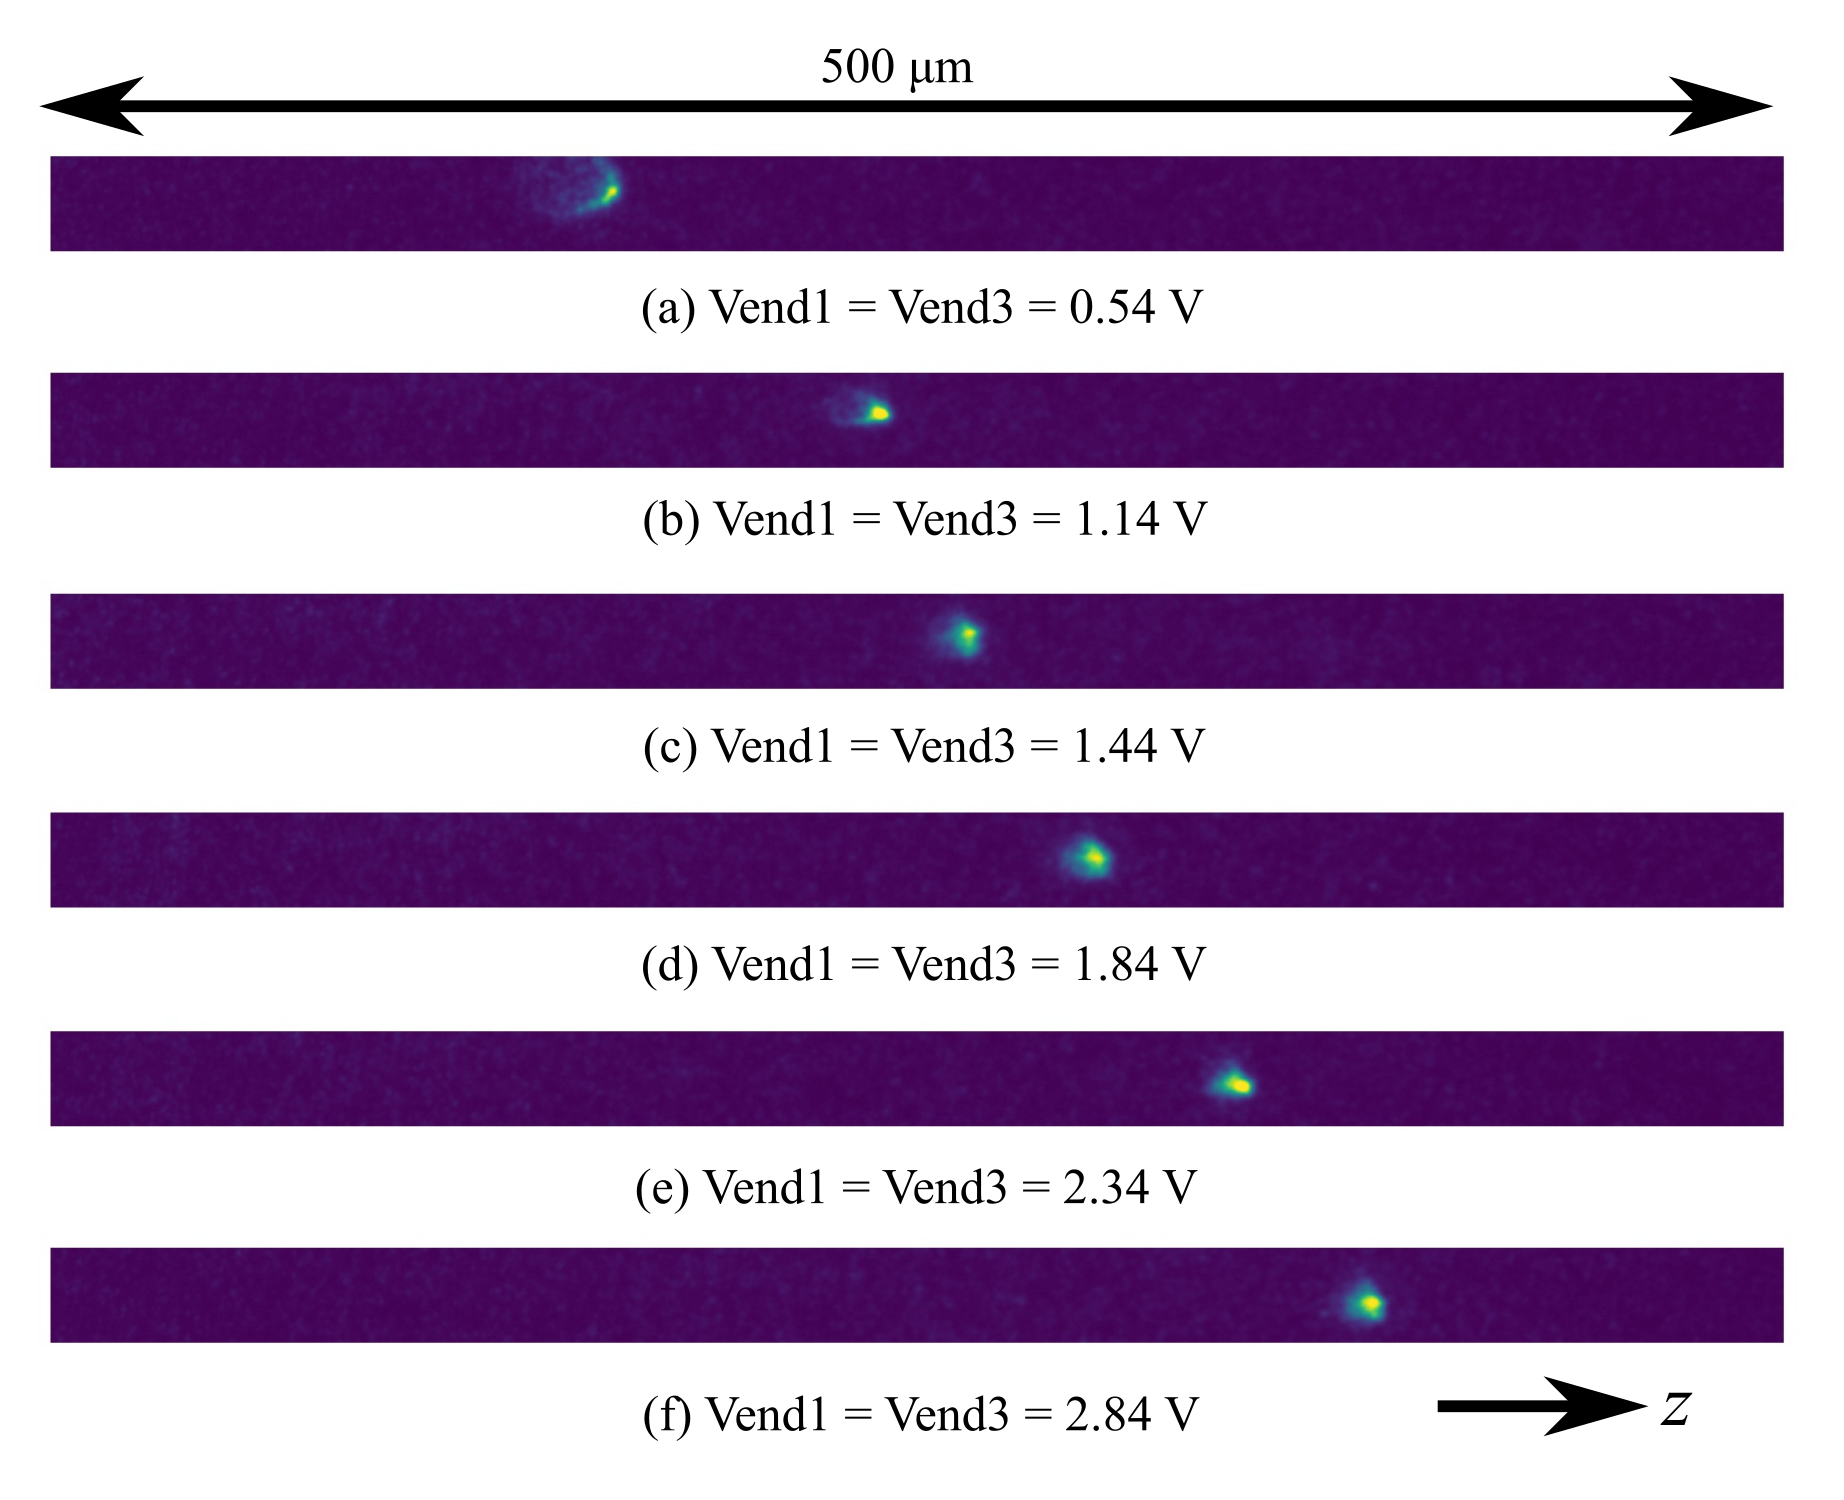
\includegraphics[width = 0.6 \linewidth]{./results/figure/displacement_End_Odd.png}
		\caption{$V_{\rm End1}, V_{\rm End3} = 0.54{\rm \ (a)}, \ 1.14{\rm \ (b)}, \ 1.44{\rm \ (c)}, \ 1.84{\rm \ (d)}, \ 2.34{\rm \ (e)}, \ 2.84{\rm \ (f)} \ {\rm V}$のときのイオン捕獲画像}
		\label{fig:displacement_End13}
	\end{center}
\end{figure}

\Fig{displacement_End13}より,End1とEnd3に印加するdc電圧が大きいとイオンの捕獲位置が$+z$方向へ変位し,小さい場合には$-z$方向へ変位することが分かる.

\clearpage

\Fig{sim_exp_displacement_End13}に実測値とシミュレーション値の比較したグラフを示す.

\begin{figure}[h]
	\begin{center}
		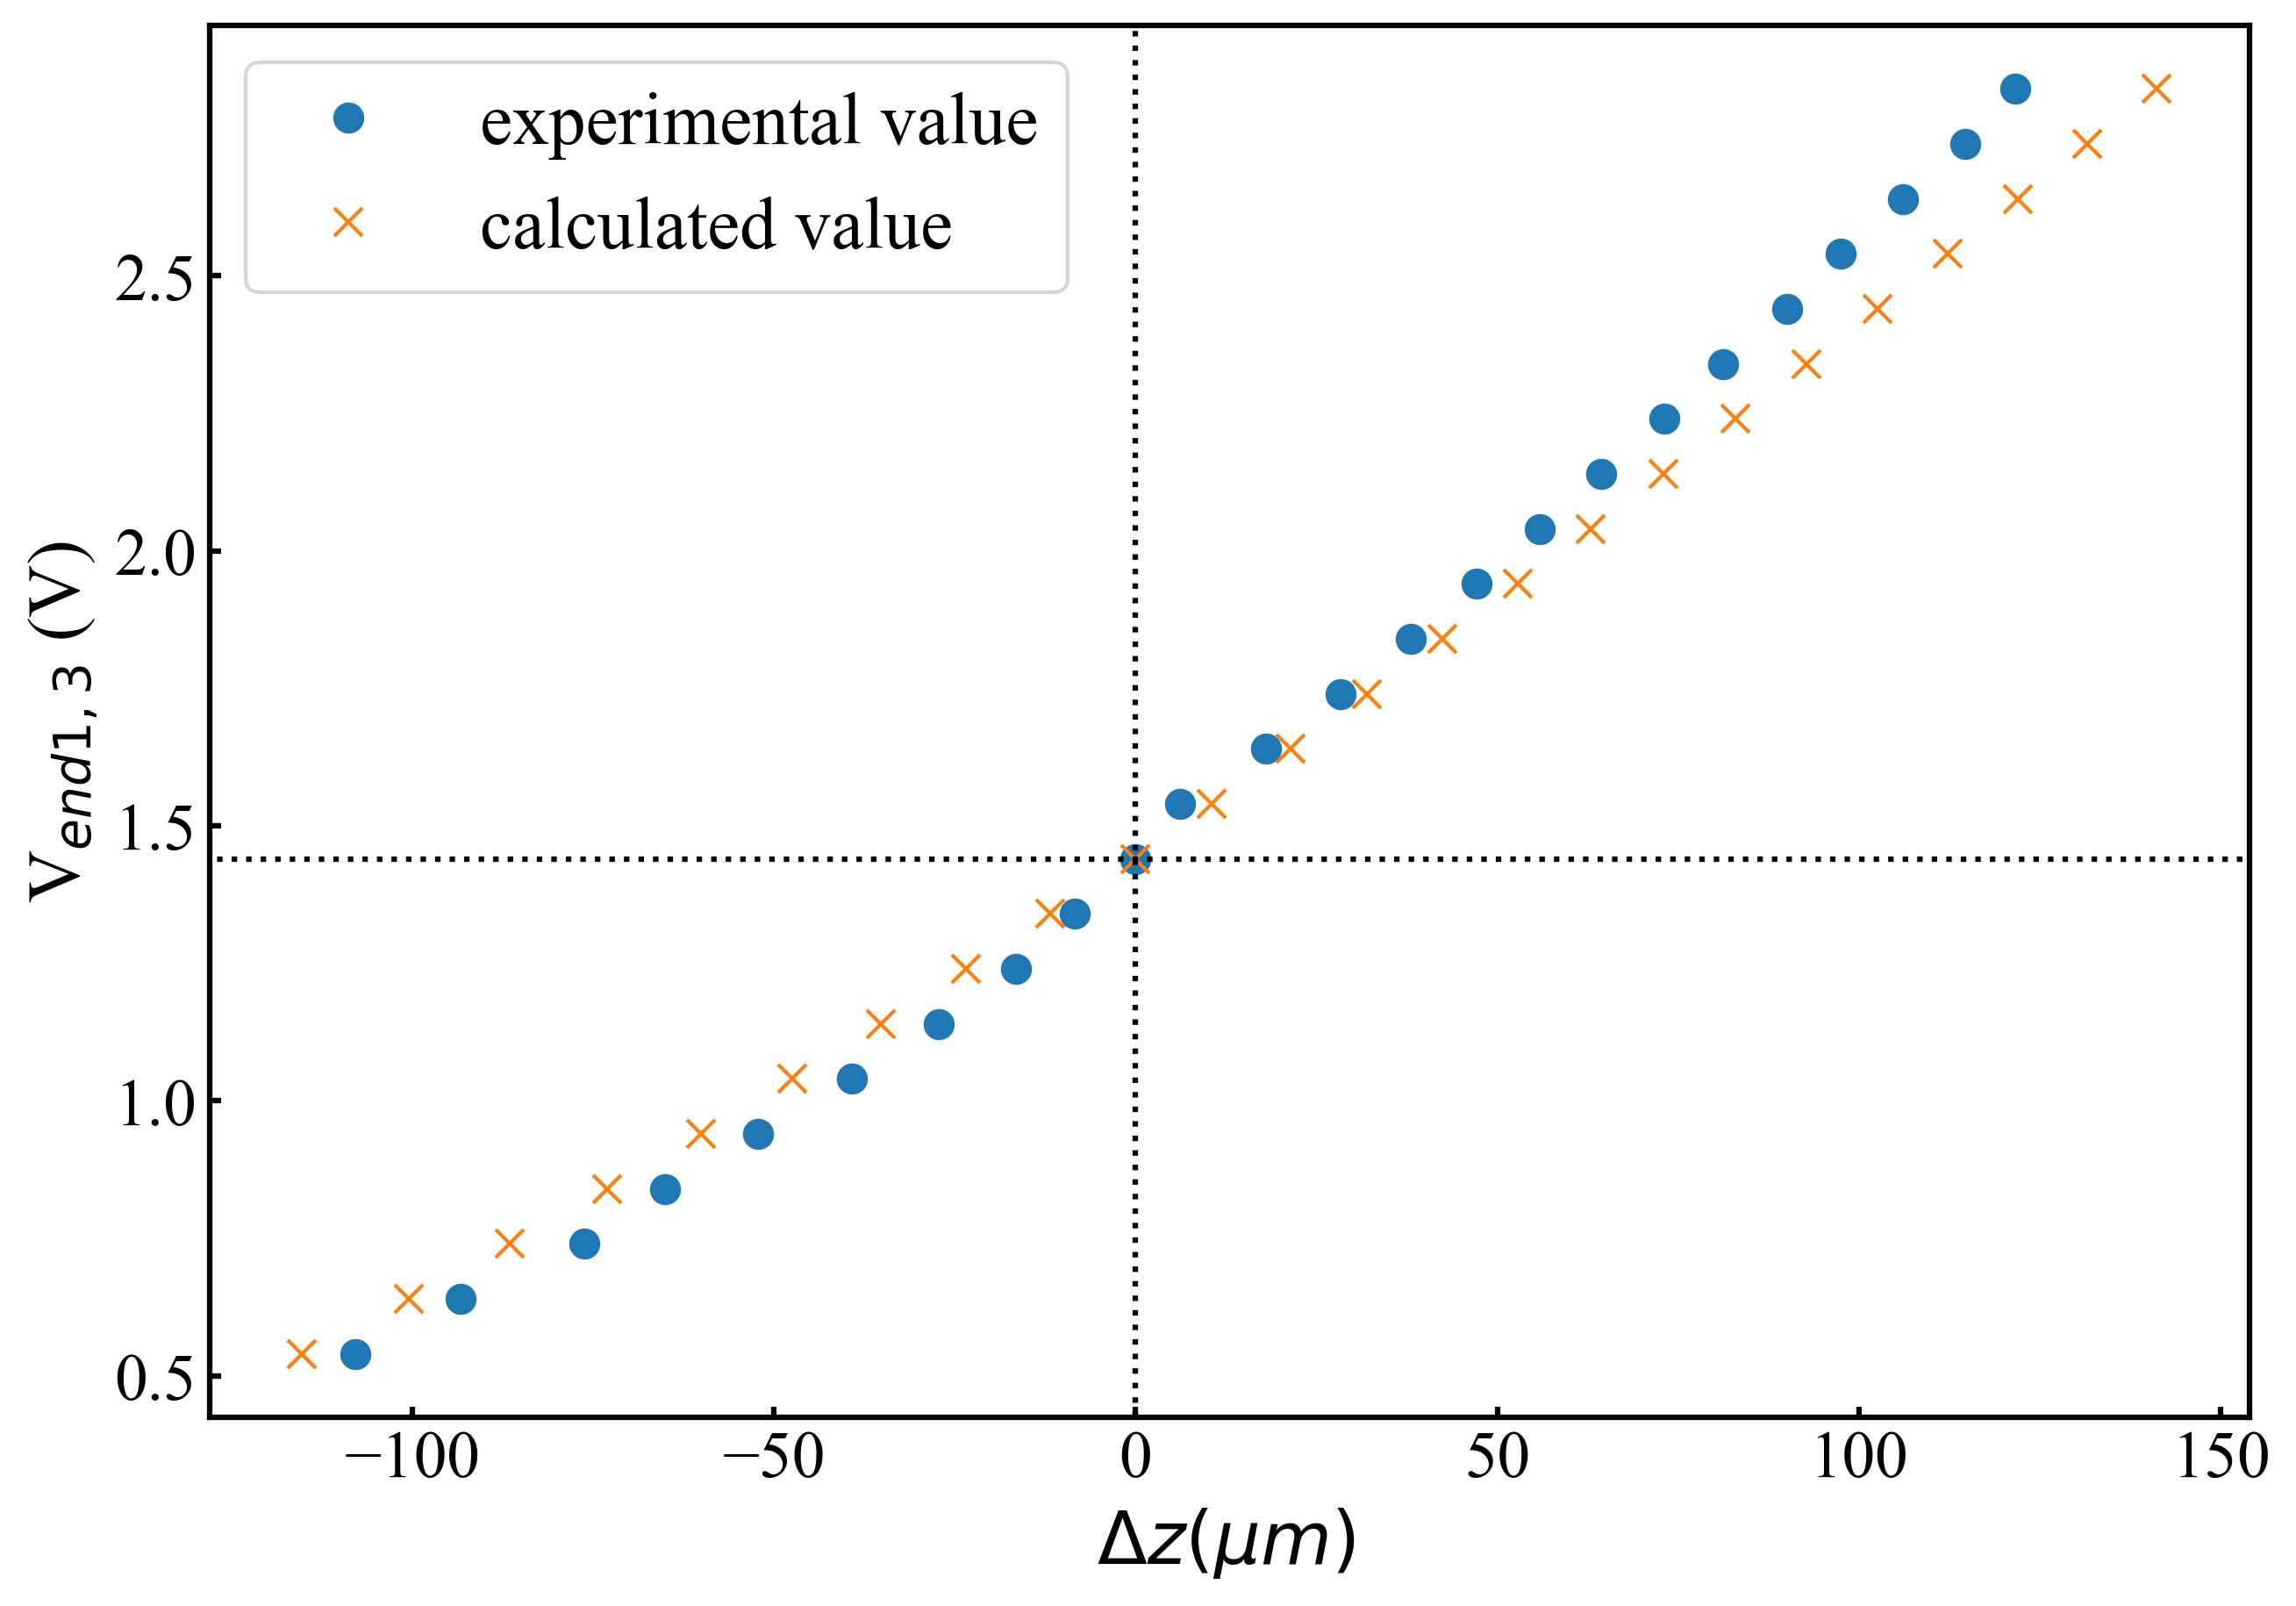
\includegraphics[width = 0.6\linewidth]{./results/figure/out_V13.jpg}
		\caption{\Tb{dc_string}の条件にて${\rm V}_{\rm End1}$と${\rm V}_{\rm End3}$の値を$0.54 \sim 2.84$Vまで0.1Vずつ変化させたときのイオン捕獲位置の変位の実測値とシミュレーション値との比較}
		\label{fig:sim_exp_displacement_End13}
	\end{center}
\end{figure}

End2とEnd4の電極に印加するdc電圧の変化に対するイオン捕獲位置の変位についても同様の実験を行った.実測値とシミュレーション値との比較を\Fig{sim_exp_displacement_End24}に示す.

\begin{figure}[h]
	\begin{center}
		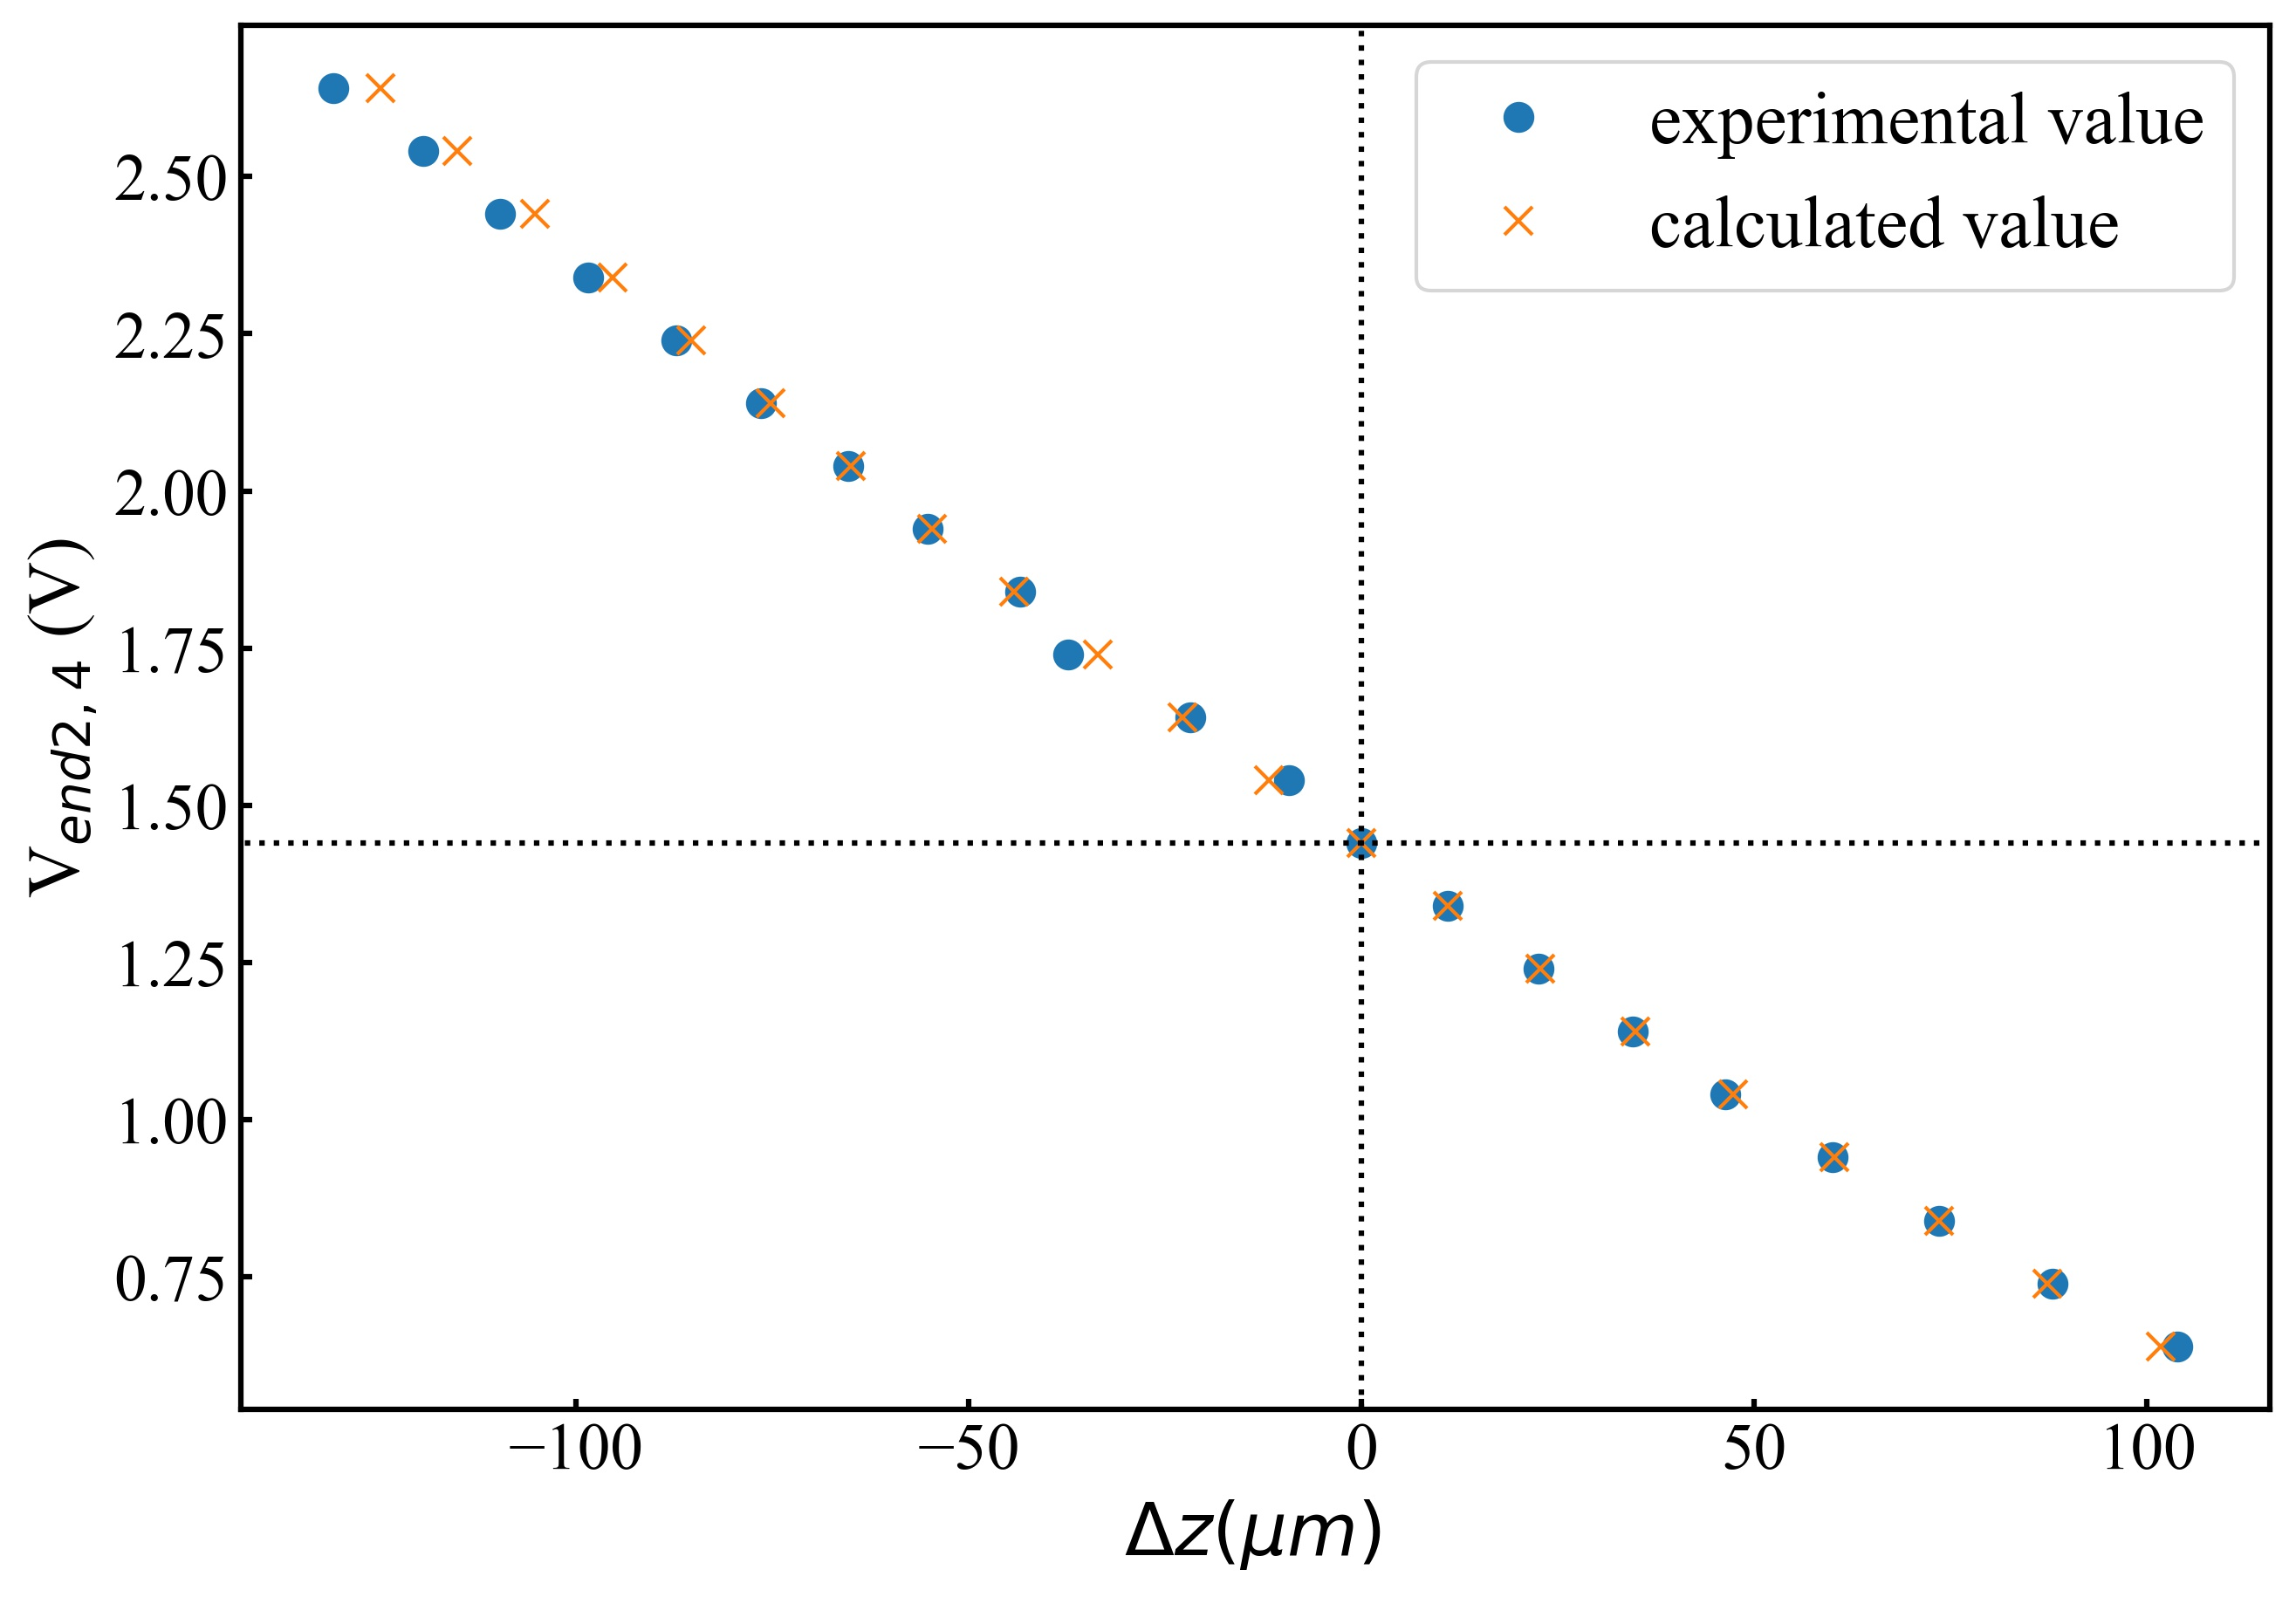
\includegraphics[width = 0.6\linewidth]{./results/figure/out_V24.jpg}
		\caption{\Tb{dc_string}の条件にて${\rm V}_{\rm End2}$と${\rm V}_{\rm End4}$の値を$0.54 \sim 2.84$Vまで0.1Vずつ変化させたときのイオン捕獲位置の変位の実測値とシミュレーション値との比較}
			\label{fig:sim_exp_displacement_End24}
	\end{center}
\end{figure}
\Fig{sim_exp_displacement_End24}より,End2とEnd4に印加するdc電圧が小さい場合に$+z$方向へイオン捕獲位置が変位し,大きい場合に$-z$方向へ変位することが確認できた.

\clearpage

\subsection{永年周波数のdc電圧依存性}
\ref{MeasSecFreq_Method}に示した手法を用いて,単一イオンを用いて異なるdc電圧セットにおける永年周波数の測定を行い,シミュレーション値との比較を行った.\Fig{end13_MeasSec}に\Tb{dc_string}を基準にして,$V_{\rm end1}, \ V_{\rm end3}$を変化させたときのイオンの振幅の周波数特性を示す.各条件に対し共鳴現象を引き起こすac信号の振幅は200$\ {\rm mV_{pp}}$とし,周波数掃引の刻み幅は50$\ {\rm Hz}$としている.周波数掃引の範囲は,まず手動で周波数を変化させ,共鳴現象が確認される周波数から$\pm1.5 \ {\rm kHz}$程度の範囲としイオンの振幅の周波数特性の取得を行った.

\begin{figure}[h]
	\begin{center}
		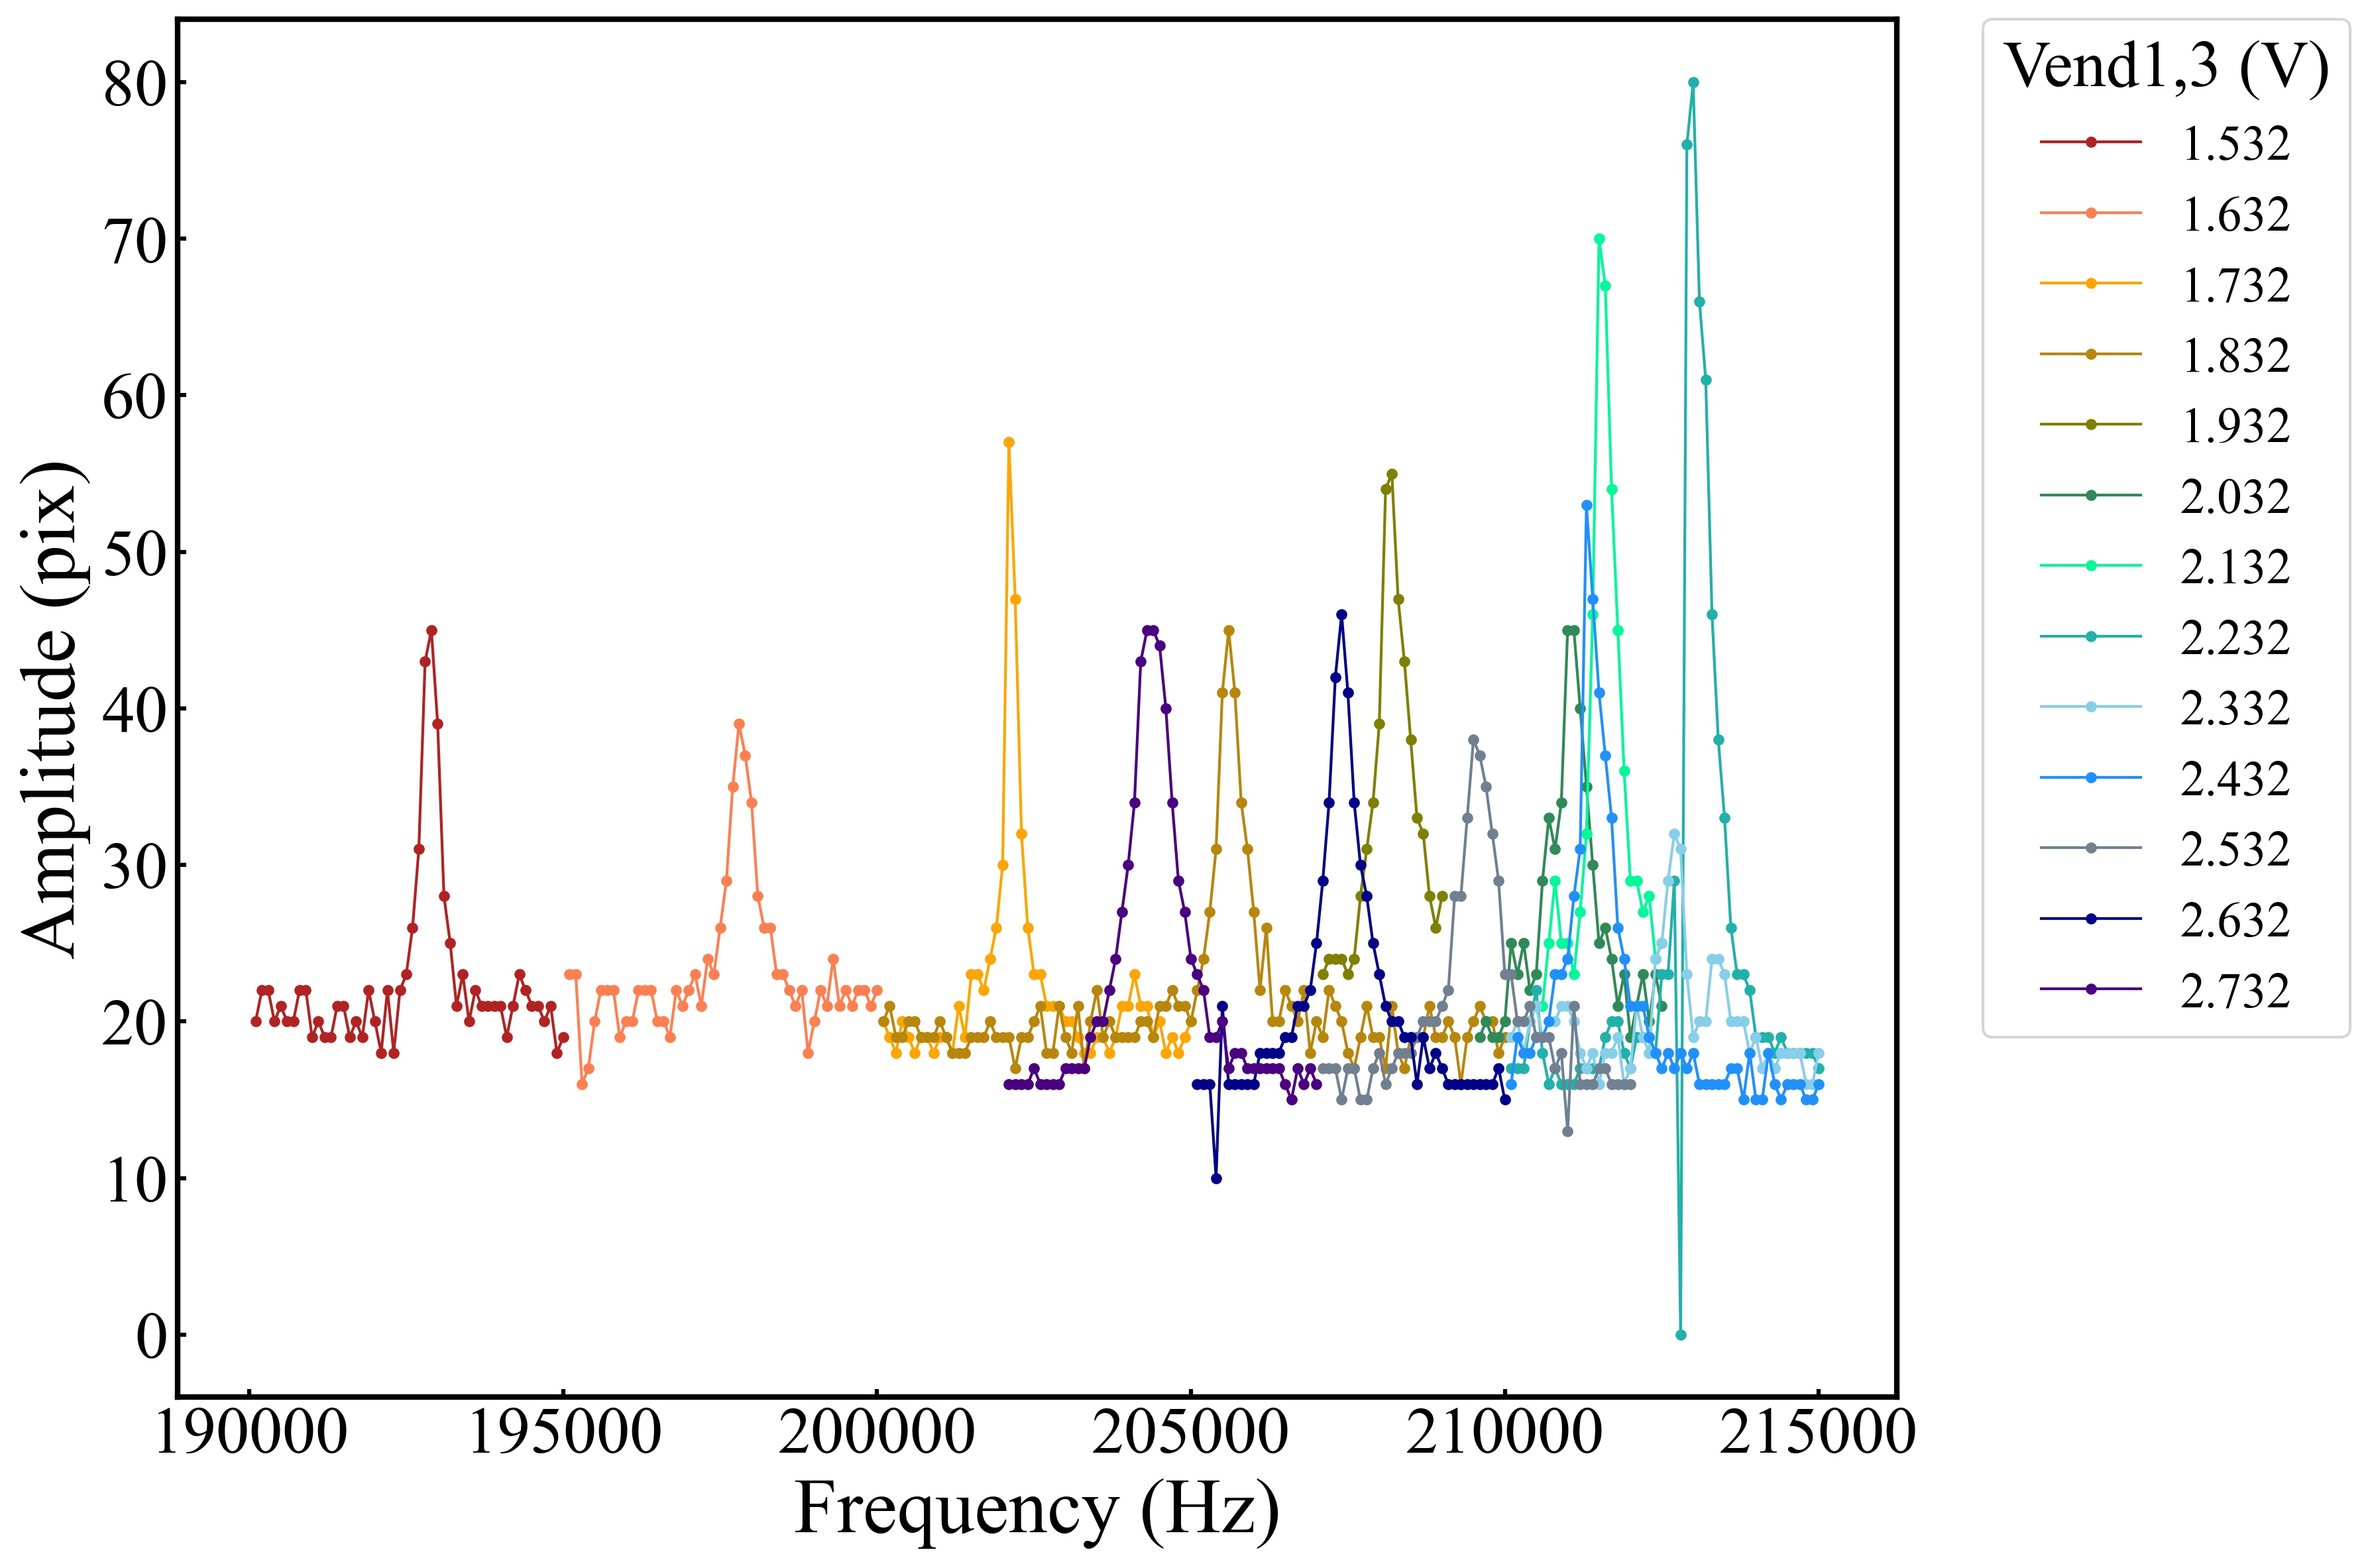
\includegraphics[width = 0.6\linewidth]{./results/figure/end13-SecFreq.jpg}
		\caption{$V_{\rm End1}$と$V_{\rm End3}$を変化させたときのイオンの振幅の周波数特性}
		\label{fig:end13_MeasSec}
	\end{center}
\end{figure}

\Fig{end13_MeasSec}より,それぞれのイオンの振幅の周波数特性をローレンツ分布関数によるフィッティングを行い,永年周波数の決定を行った.フィッティングで得られた永年周波数とシミュレーションから計算された永年周波数との比較を\Fig{end13_MeasSec_SimSec}に示す.

\begin{figure}[h]
	\begin{center}
		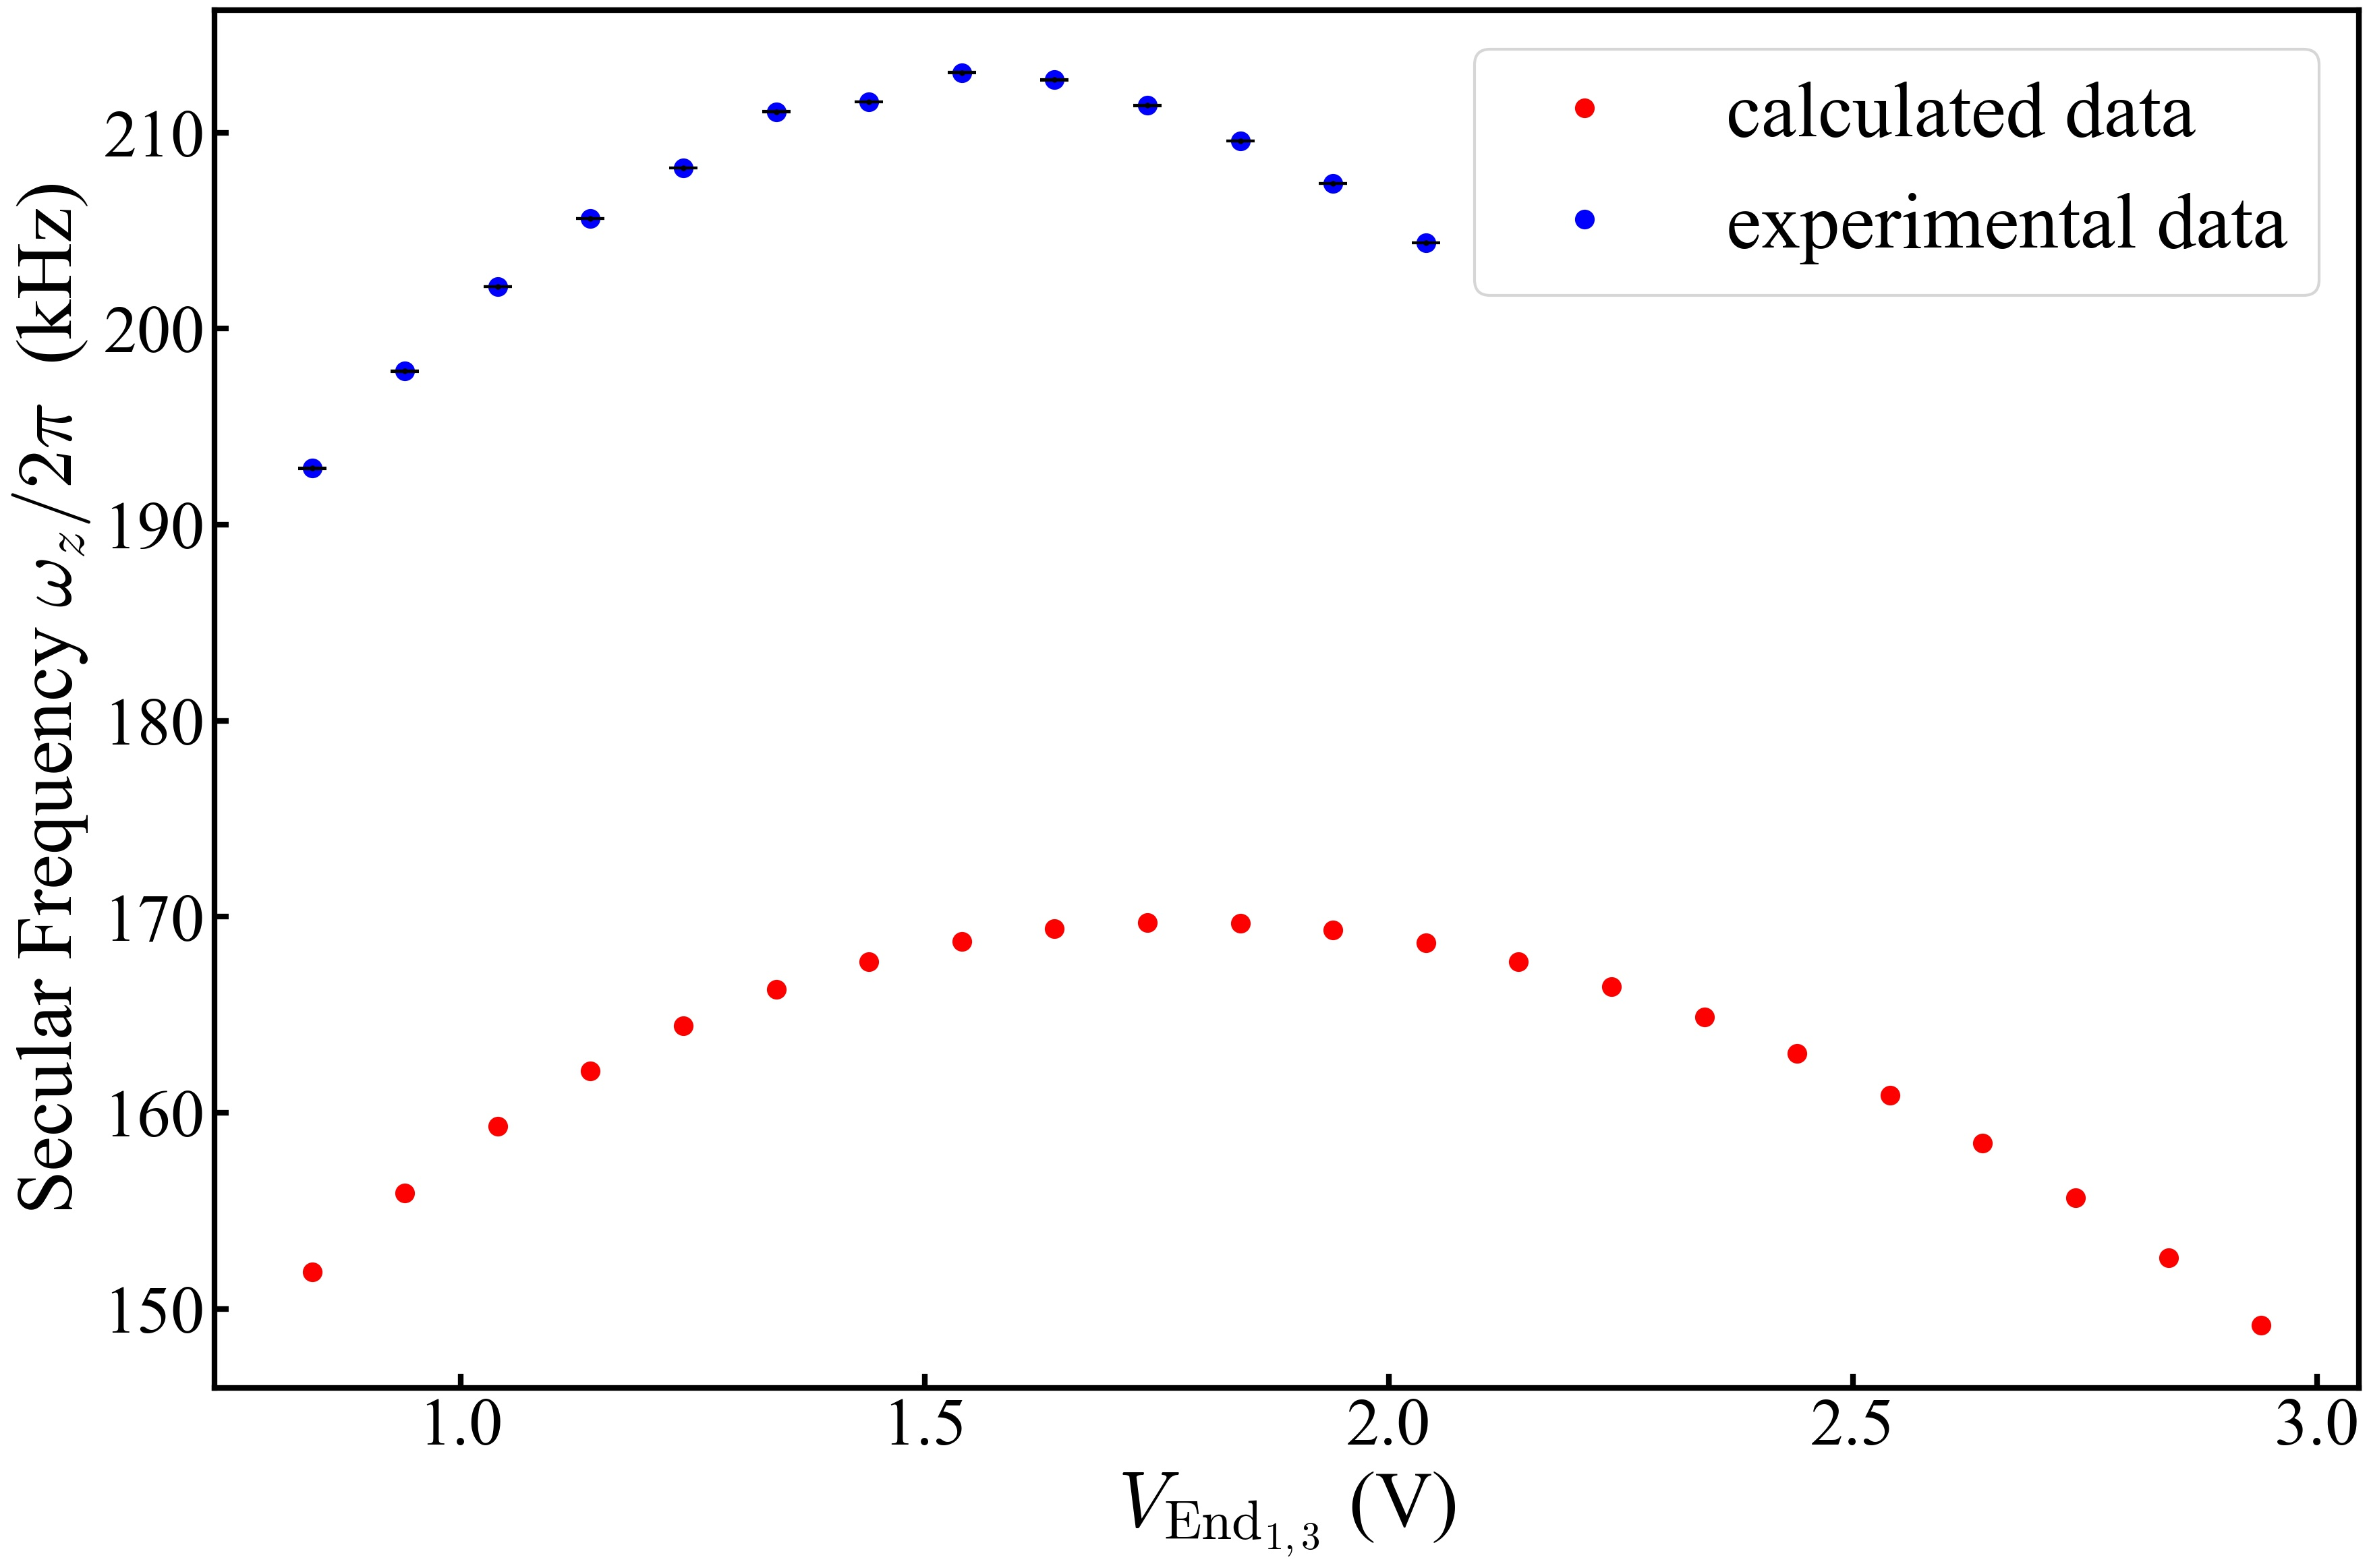
\includegraphics[width = 0.6\linewidth]{./results/figure/Vend13-SecFreqZ.jpg}
		\caption{$V_{\rm End1}$と$V_{\rm End3}$を変化させたときの永年周波数の測定結果とシミュレーション結果との比較}
		\label{fig:end13_MeasSec_SimSec}
	\end{center}
\end{figure}

\Fig{end13_MeasSec_SimSec}より,測定値とシミュレーション値との差が$35.726 \ {\rm kHz} \ \sim 44.771 \ {\rm kHz}$の範囲で存在することが分かる.また,永年周波数の$V_{\rm End1}$と$V_{\rm End3}$依存性における極値を取る$V_{\rm End1}, \ V_{\rm End3}$が異なっていることが分かる.

次に,$V_{\rm End2}$と$V_{\rm End4}$を変化させ,同様の手順で永年周波数の測定を行った.このときのイオンの振幅の周波数特性を\Fig{end24_MeasSec}に示す.

\begin{figure}[h]
	\begin{center}
		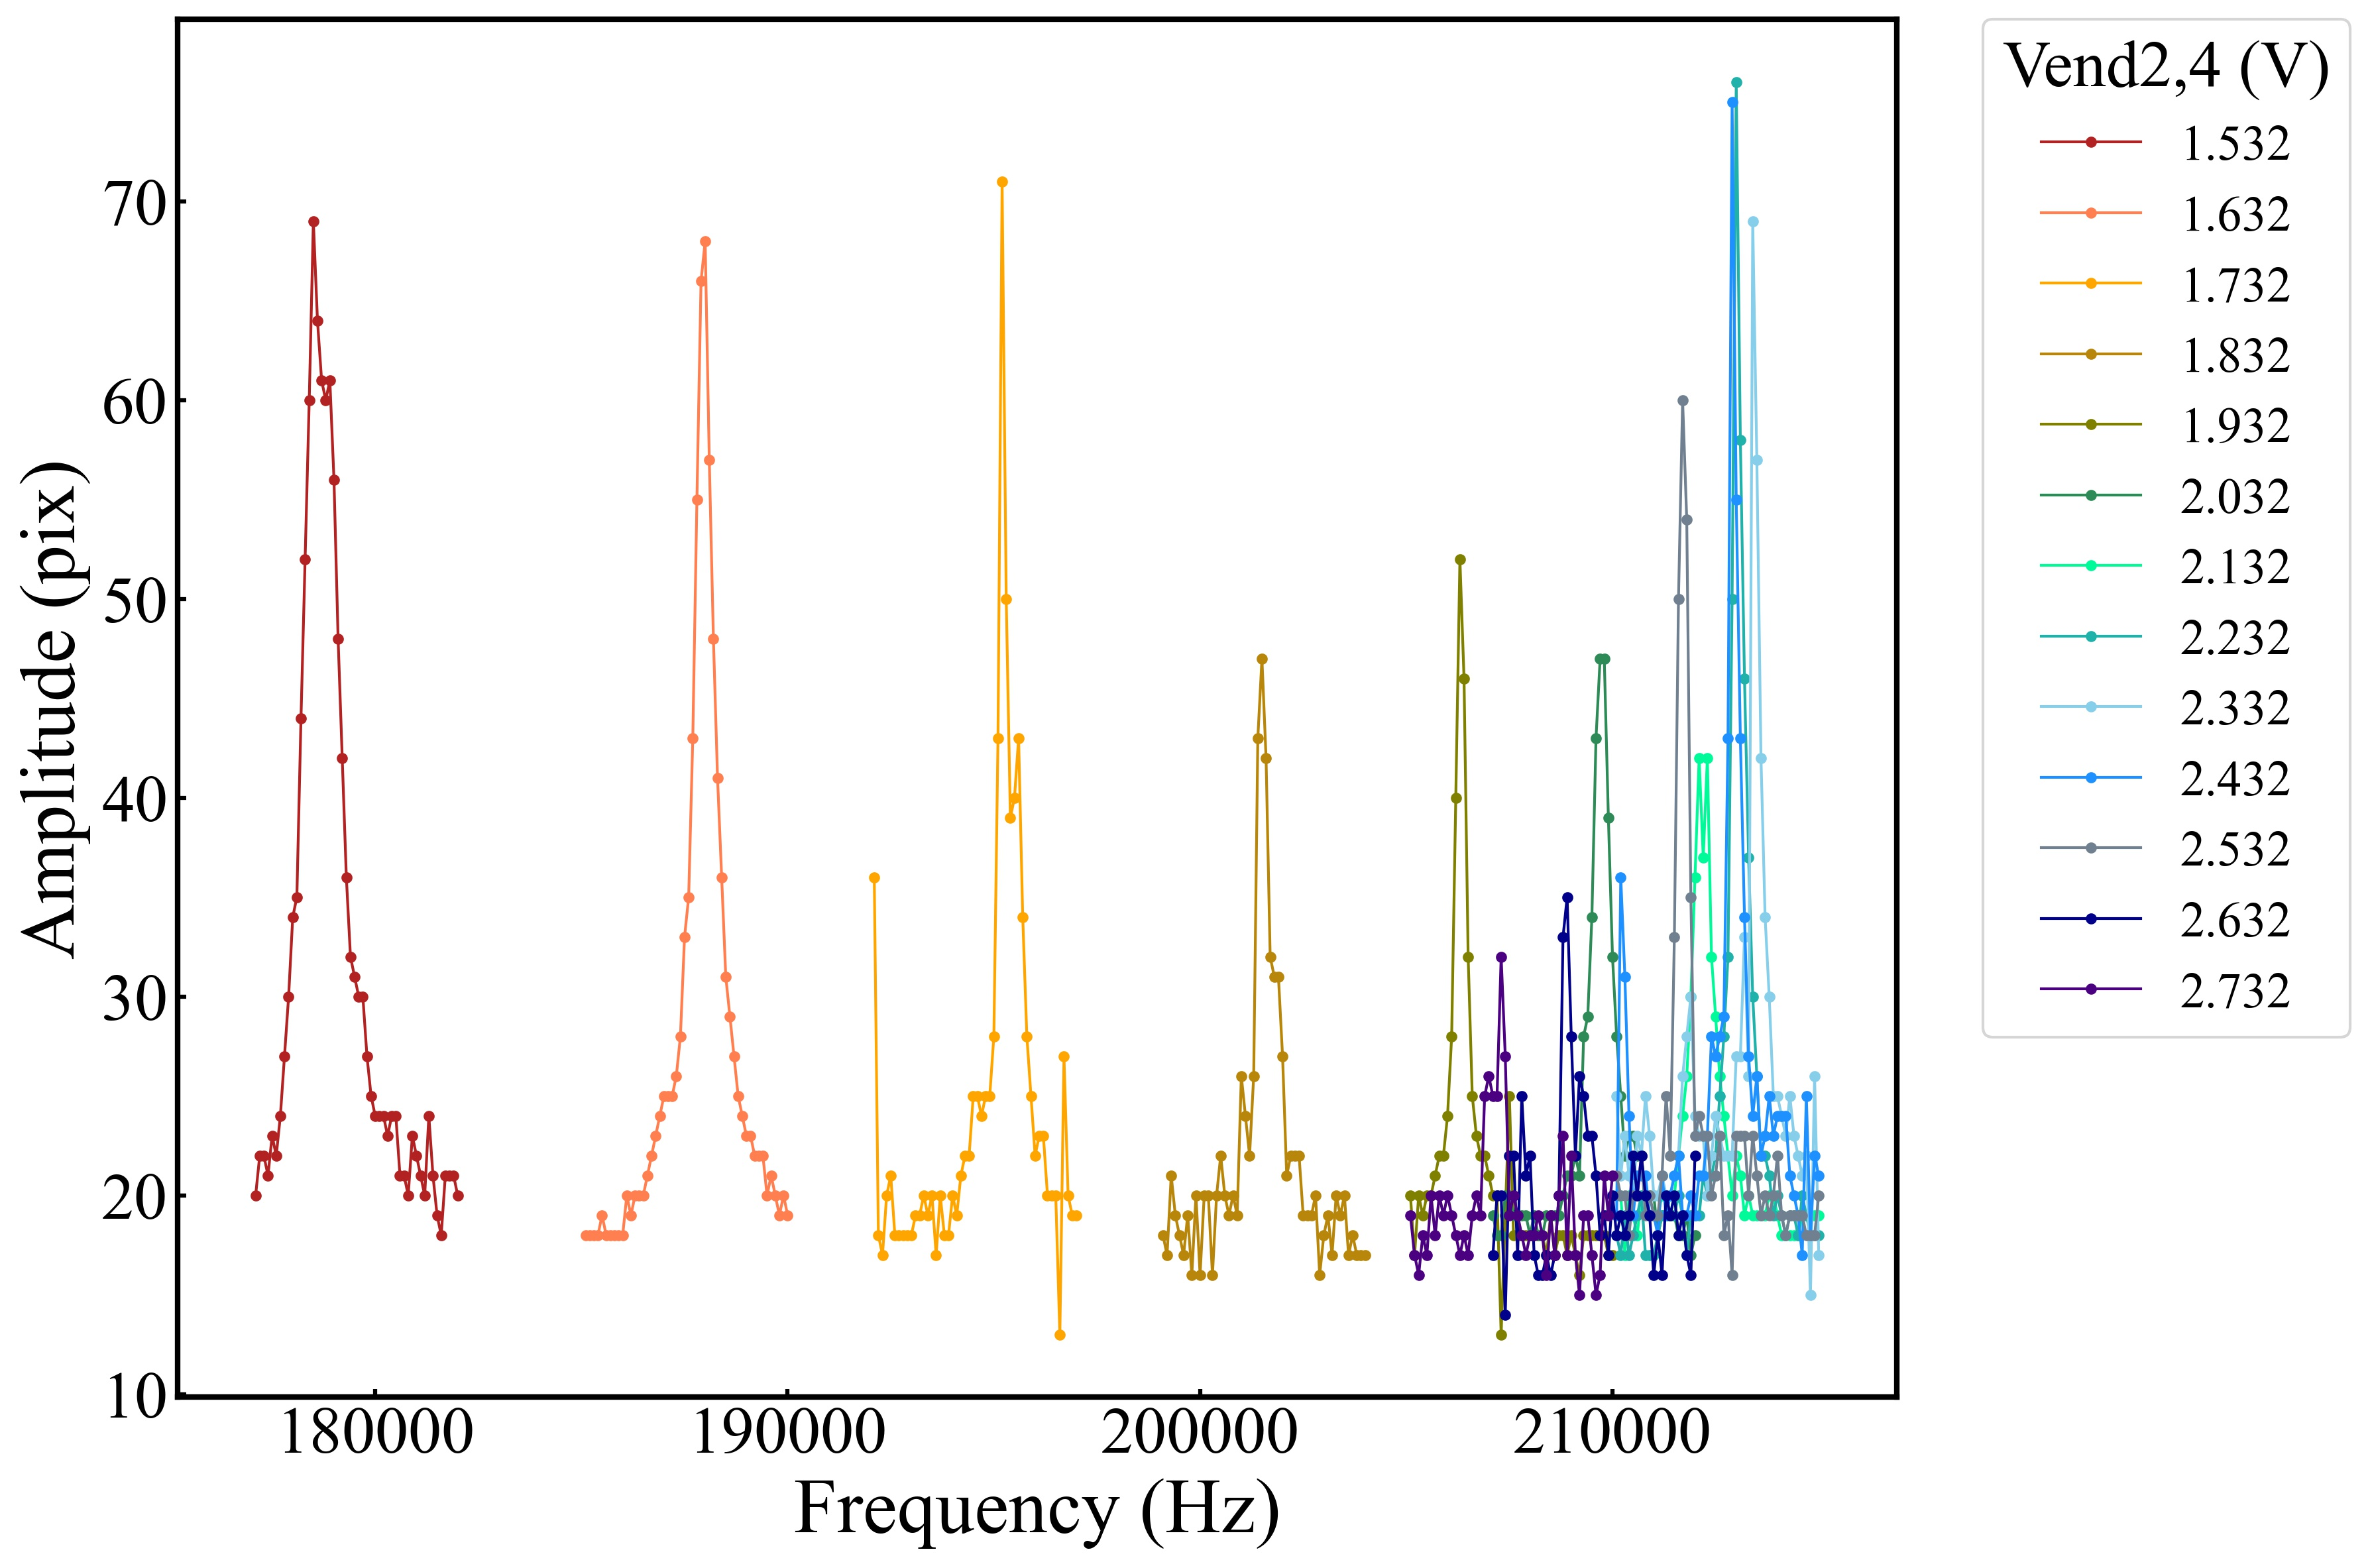
\includegraphics[width = 0.6\linewidth]{./results/figure/end24-SecFreq.jpg}
		\caption{$V_{\rm End2}$と$V_{\rm End4}$を変化させたときのイオンの振幅の周波数特性}
		\label{fig:end24_MeasSec}
	\end{center}
\end{figure}

\Fig{end24_MeasSec}より,ローレンツ分布関数によるフィッティングから得られた永年周波数とシミュレーションから得られた永年周波数との比較を\Fig{end24_MeasSec_SimSec}に示す.

\begin{figure}[h]
	\begin{center}
		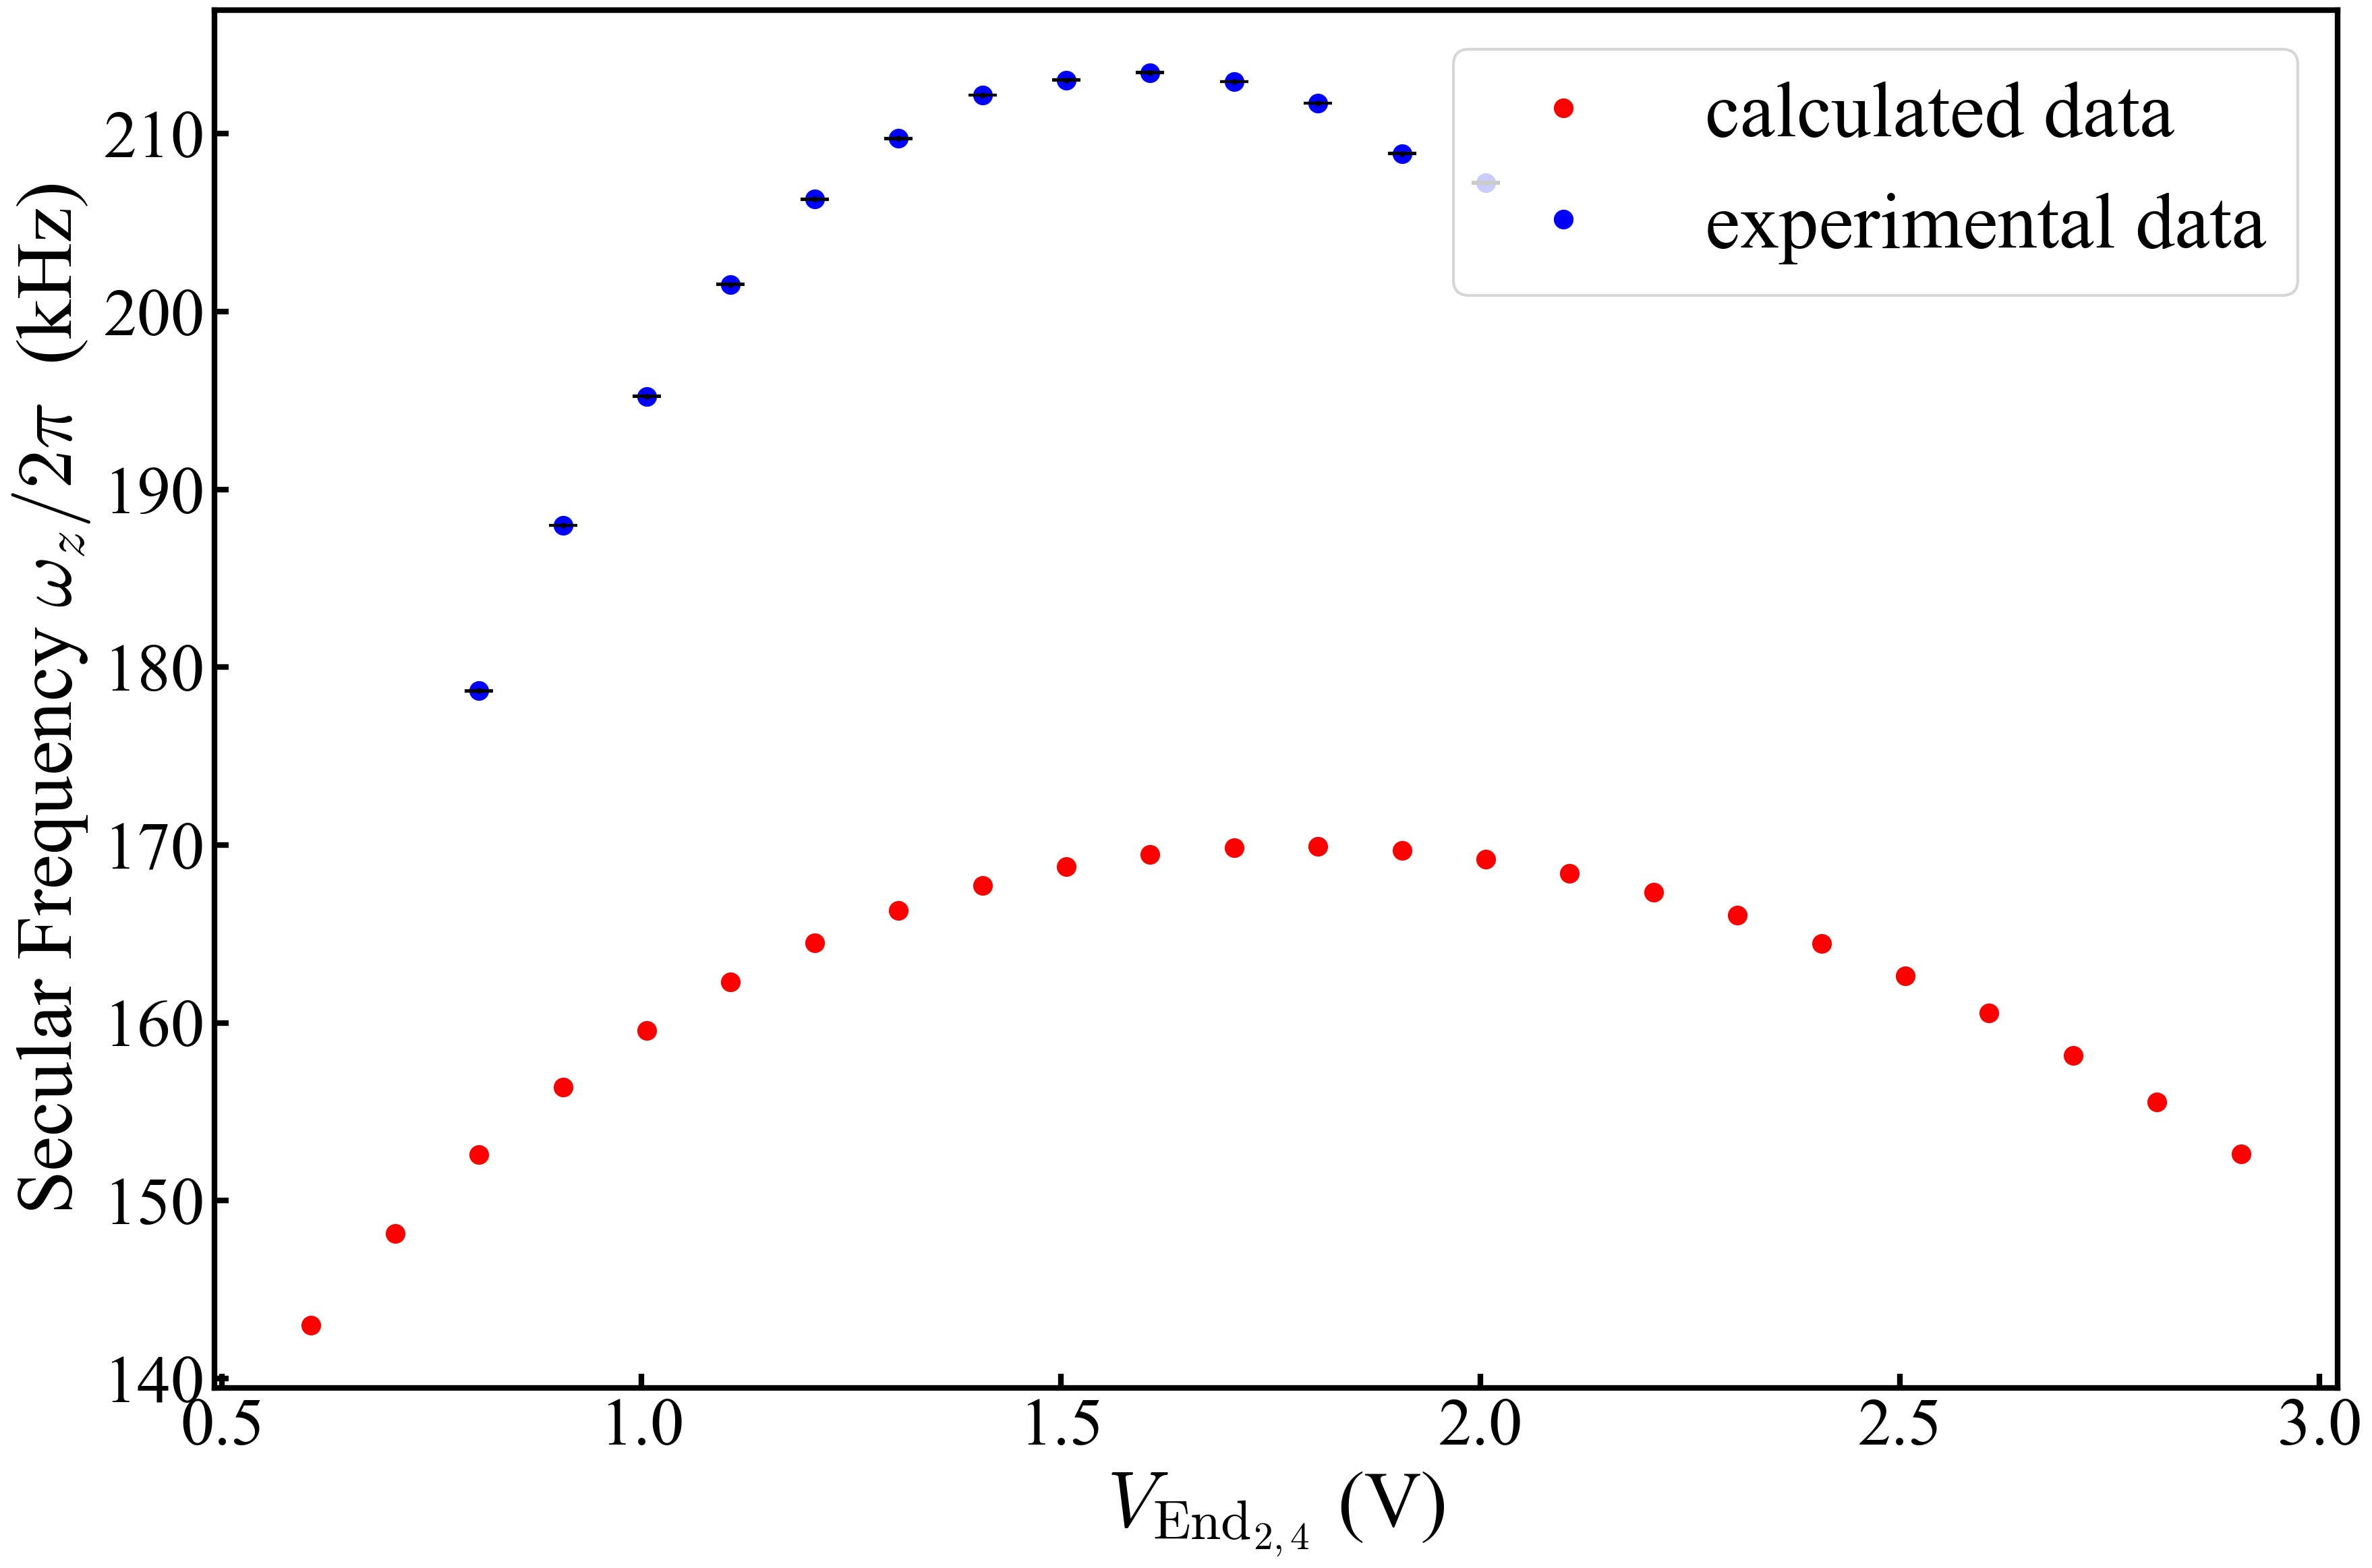
\includegraphics[width = 0.6\linewidth]{./results/figure/Vend24-SecFreqZ.jpg}
		\caption{$V_{\rm End2}$と$V_{\rm End4}$を変化させたときの永年周波数の測定結果とシミュレーション結果との比較}
		\label{fig:end24_MeasSec_SimSec}
	\end{center}
\end{figure}

\Fig{end24_MeasSec_SimSec}から,実験値とシミュレーション値に$26.1 \ {\rm kHz} \ \sim \ 44.5 \ {\rm kHz}$の差があることが分かった.また,$V_{\rm end1}, \ V_{\rm end3}$に対して変化する永年周波数と同様に実験値とシミュレーション値のそれぞれが極値を取る$V_{\rm end2}, \ V_{\rm end4}$が異なることが分かる.

\clearpage

\begin{figure}[h]
	\begin{minipage}{0.5\linewidth}
		\begin{center}
			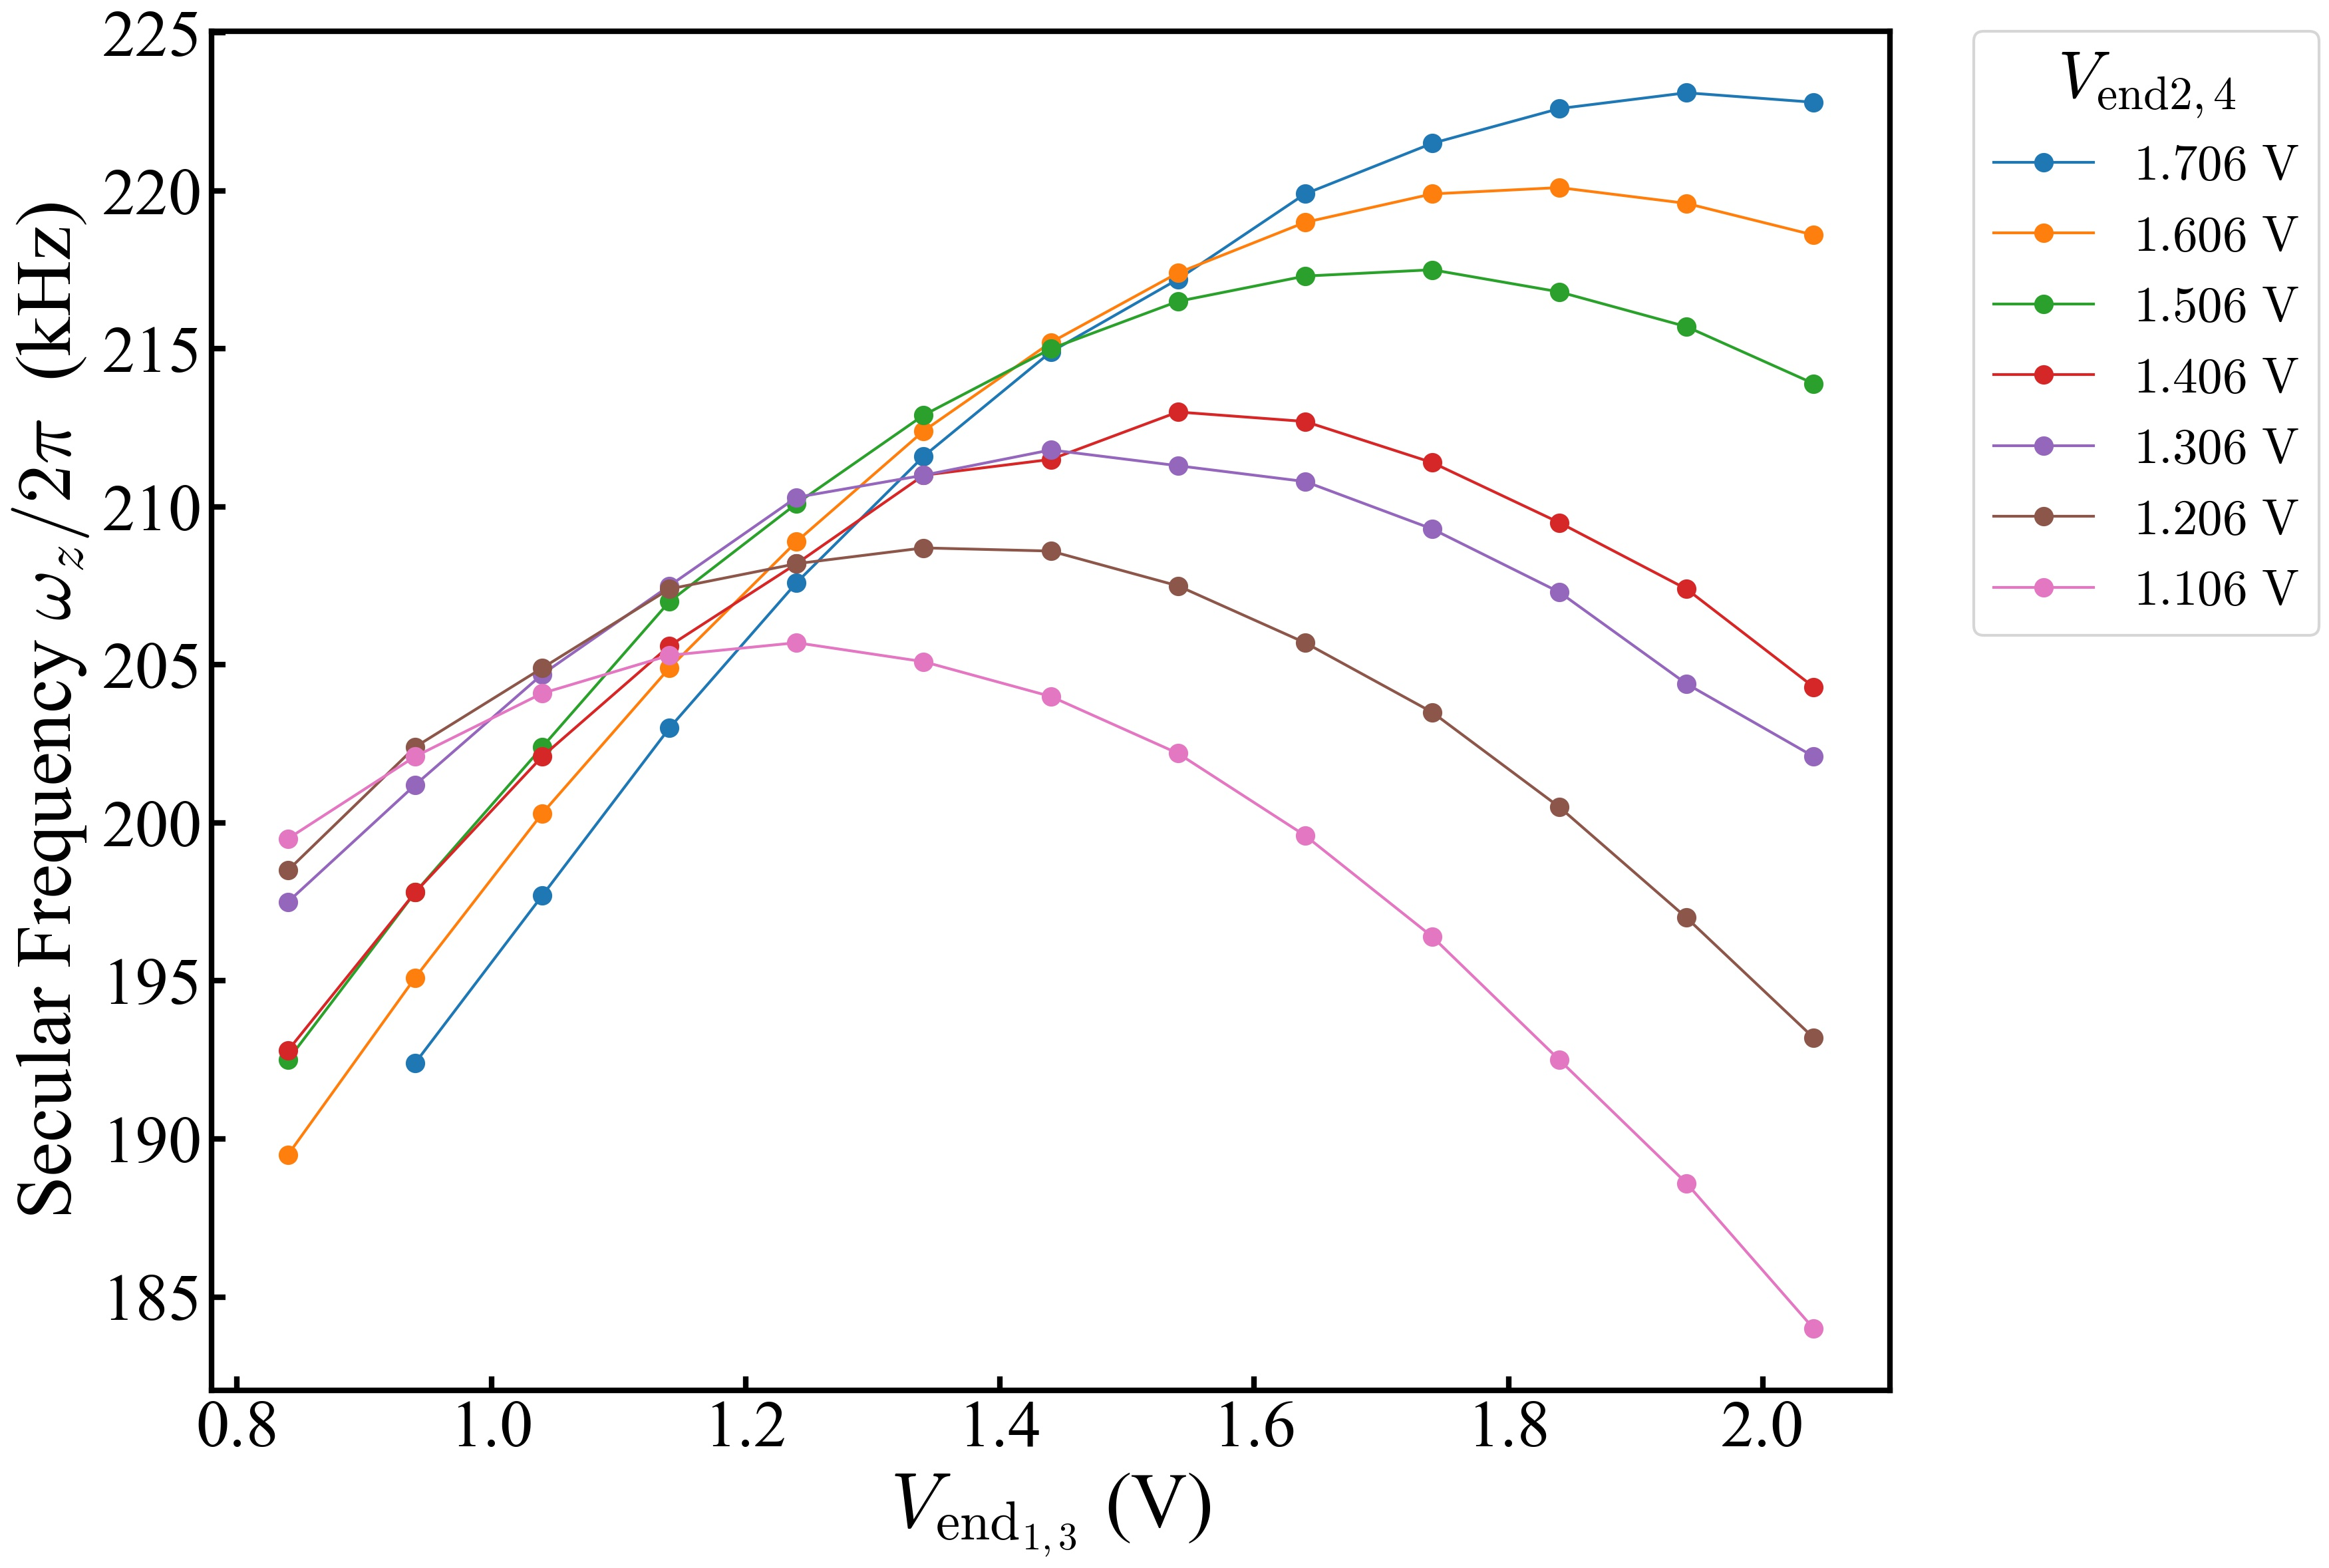
\includegraphics[width = 0.98\columnwidth]{./results/figure/Vendodd-SecFreqZ_Vendeven.jpg}
			\caption{\Fig{end13_MeasSec}と\Fig{end24_MeasSec}から得られた永年周波数の実験値}
			\label{fig:Vendodd_Vendeven}
		\end{center}
	\end{minipage}
	\begin{minipage}{0.5\linewidth}
		\begin{center}
			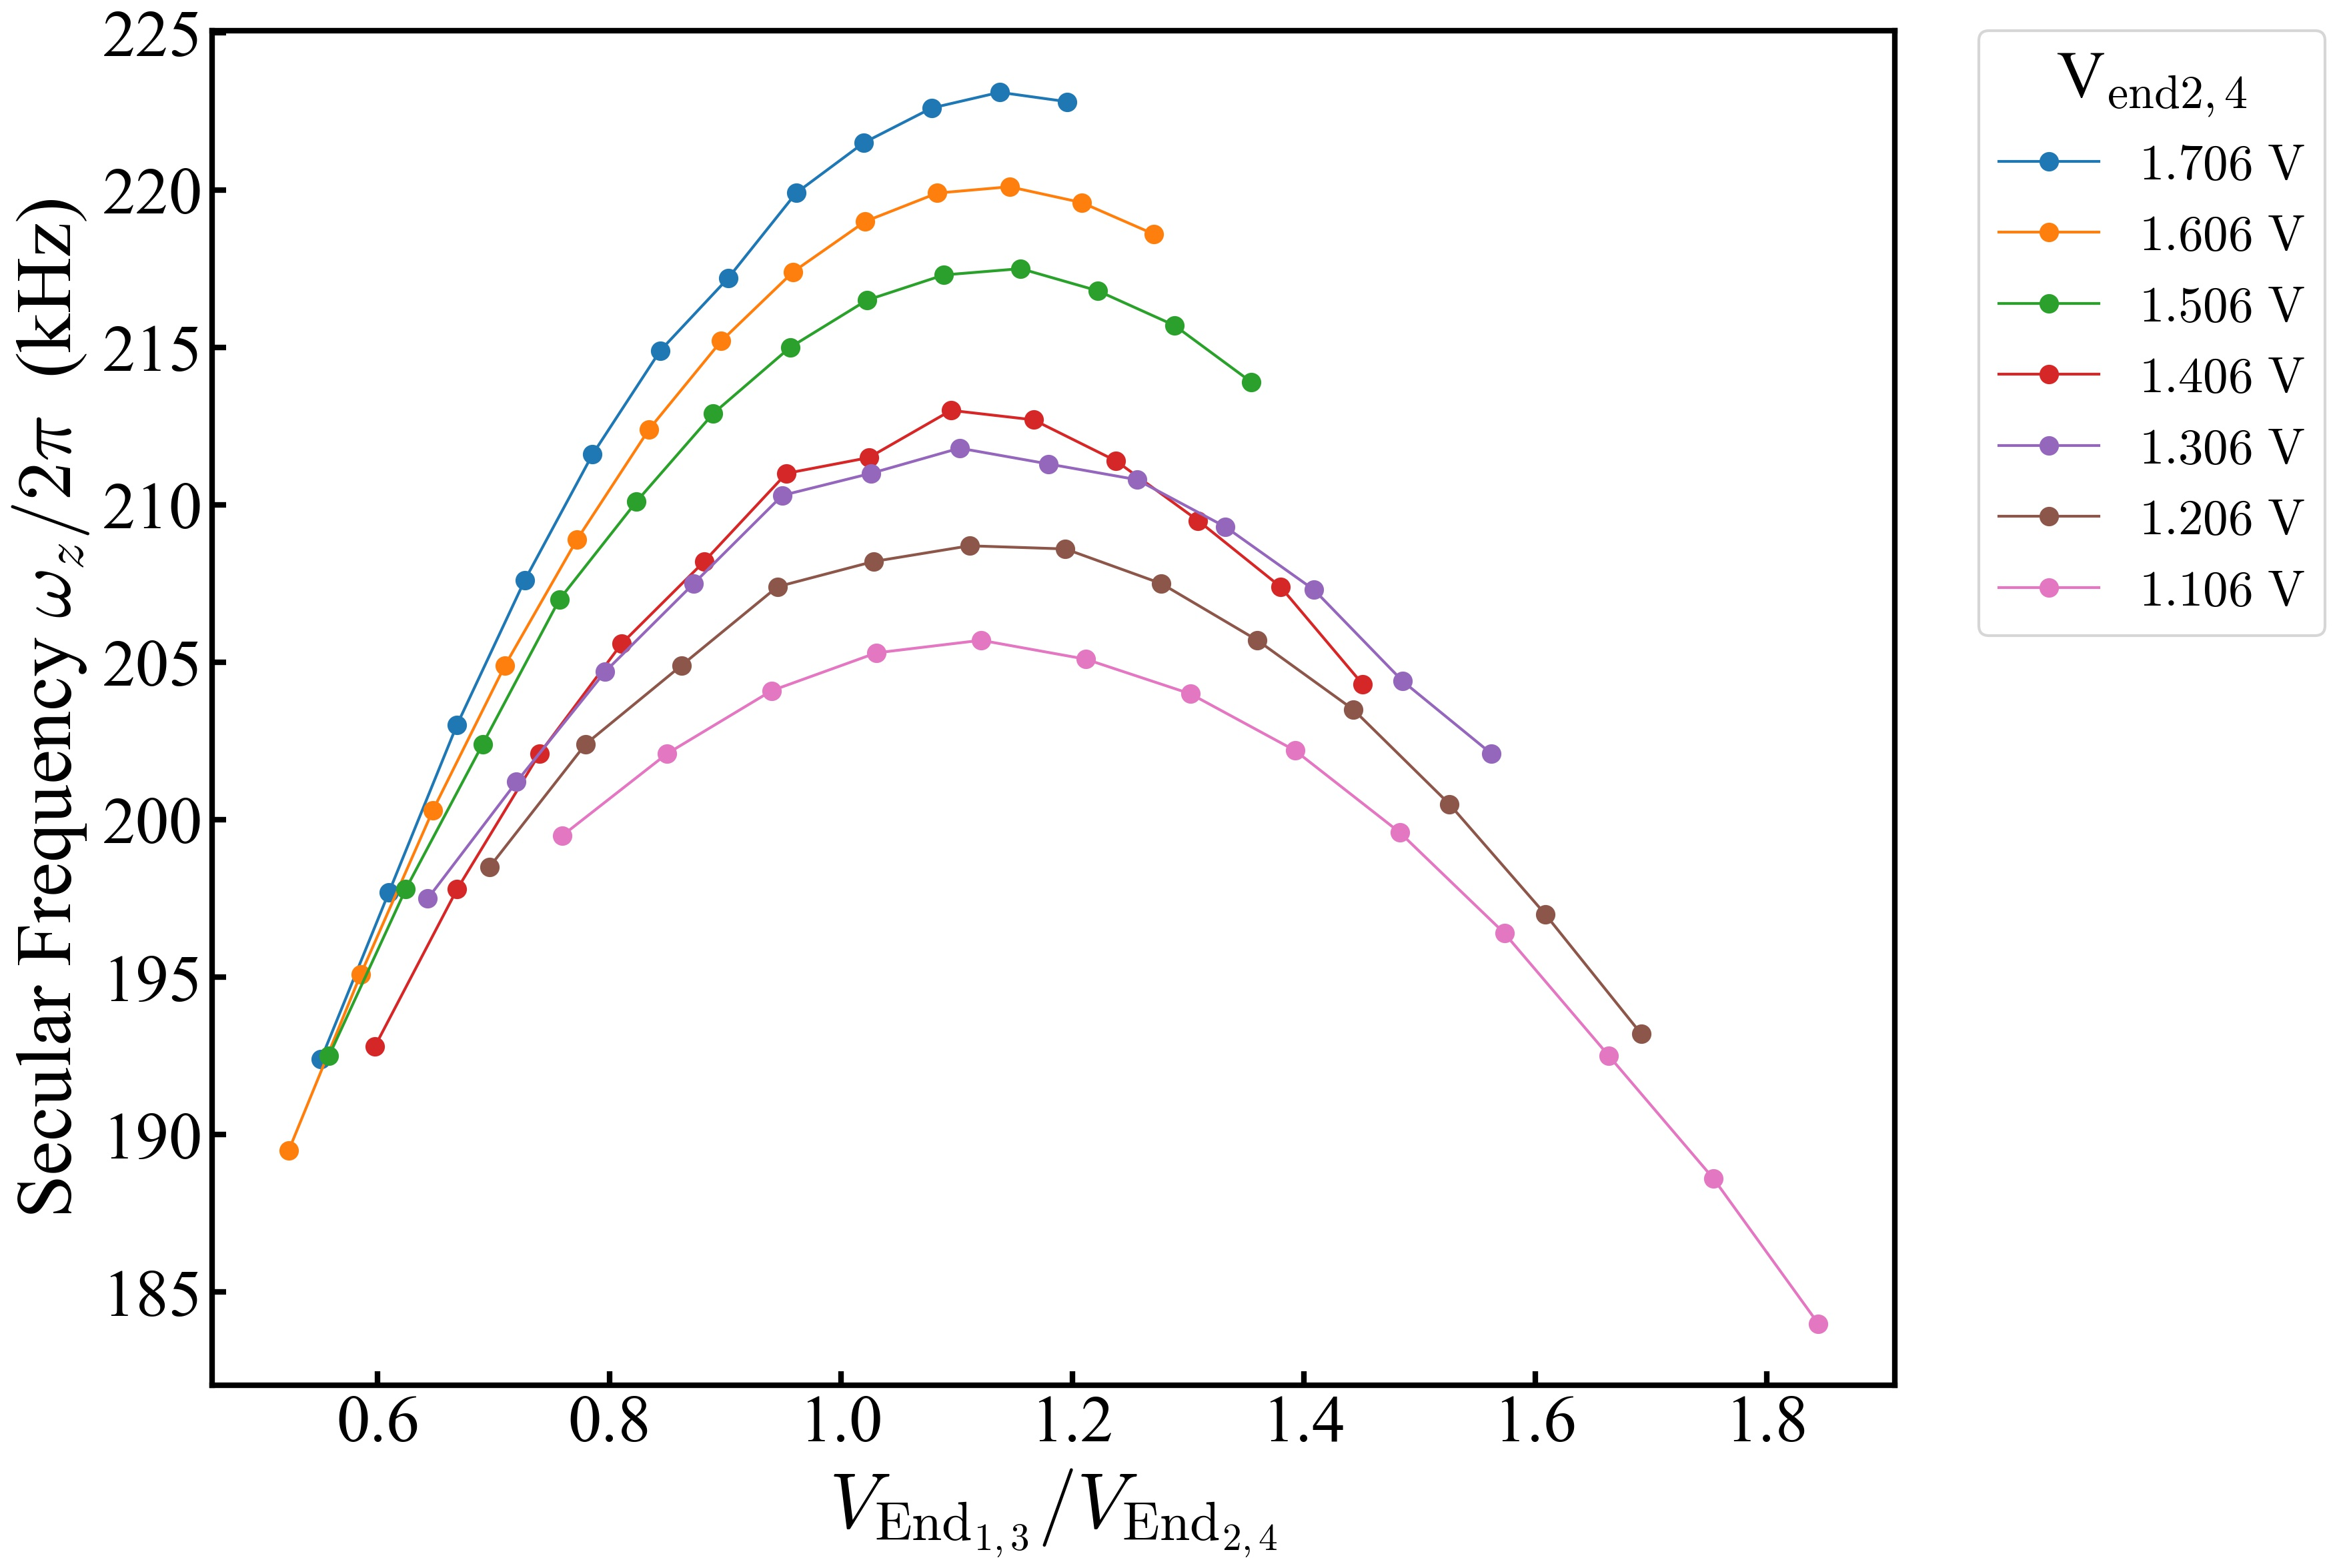
\includegraphics[width = 0.98\columnwidth]{./results/figure/Vendodd_Vendeven-SecFreqZ_.jpg}
			\caption{\Fig{Vendodd_Vendeven}において横軸に$V_{\rm end1,3}/V_{\rm end2,4}$の比率を取った場合の永年周波数の実験値}
			\label{fig:Vendodd_Vendeven_f}
		\end{center}
	\end{minipage}
\end{figure}

\begin{figure}[h]
	\begin{center}
		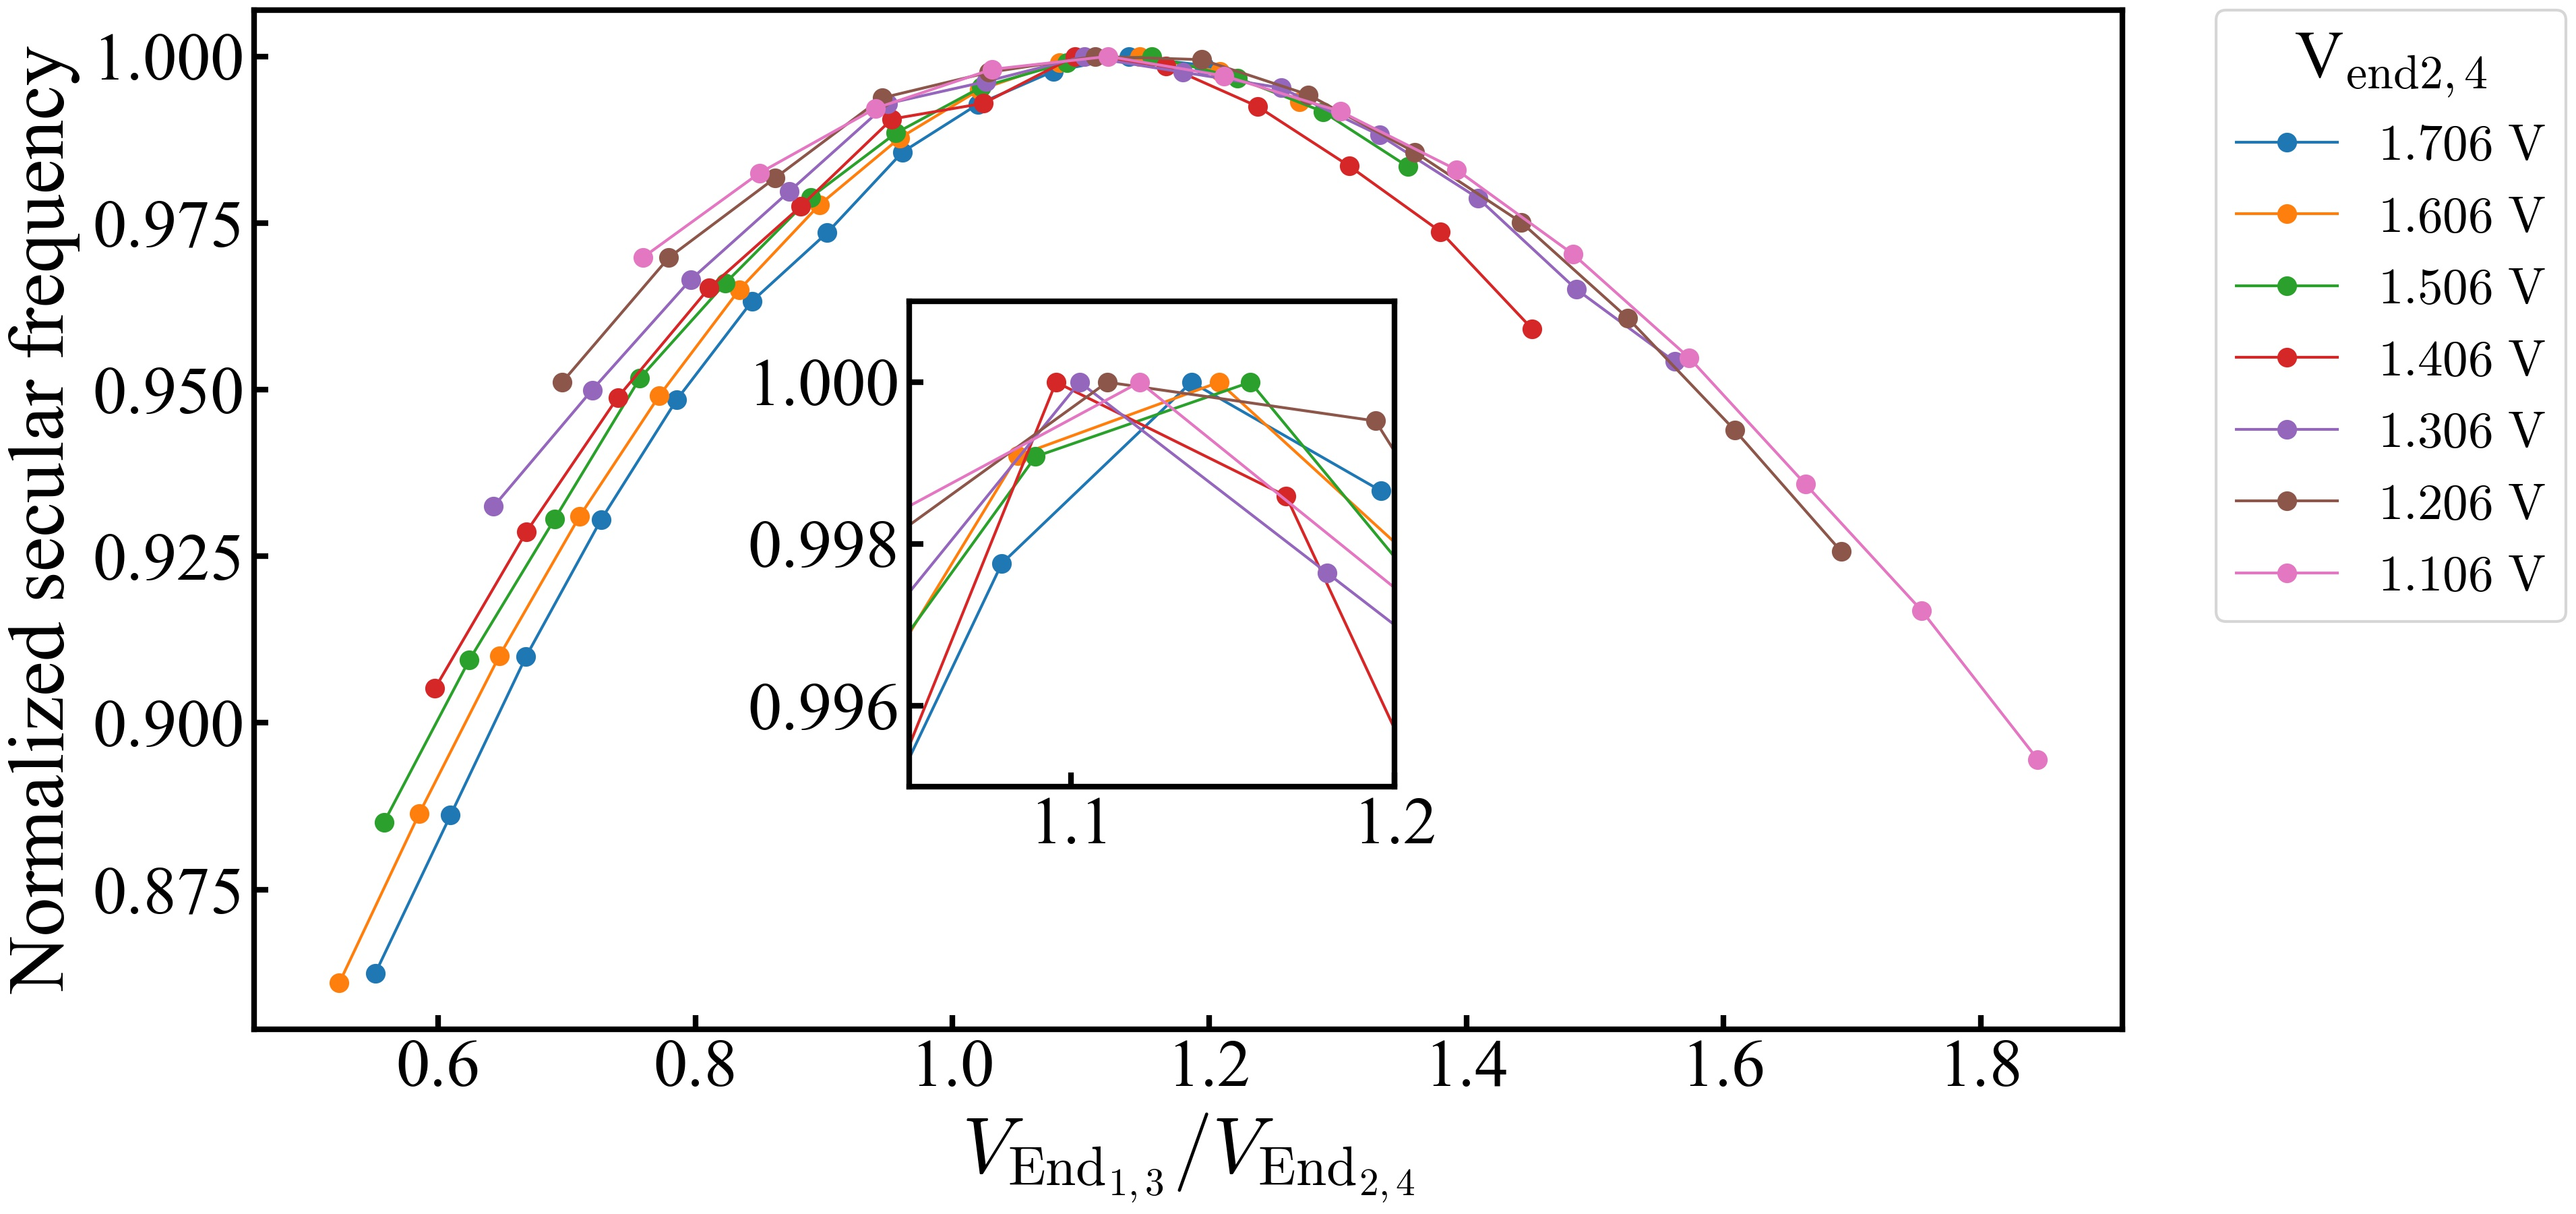
\includegraphics[width = 0.7\linewidth]{./results/figure/Normalized_Vendodd_Vendeven-SecFreqZ_.jpg}
		\caption{\Fig{Vendodd_Vendeven_f}において,$V_{\rm end2,4}$のそれぞれの条件における永年周波数で規格化した場合の永年周波数のf依存性}
		\label{fig:Norm_Vendodd_Vendeven}
	\end{center}
\end{figure}

\clearpage

最後に,$V_{\rm middle1}, \ V_{\rm middle2}$を変化させた場合のイオンの振幅の周波数特性を\Fig{mid_MeasSec}に示す.

\begin{figure}[h]
	\begin{center}
		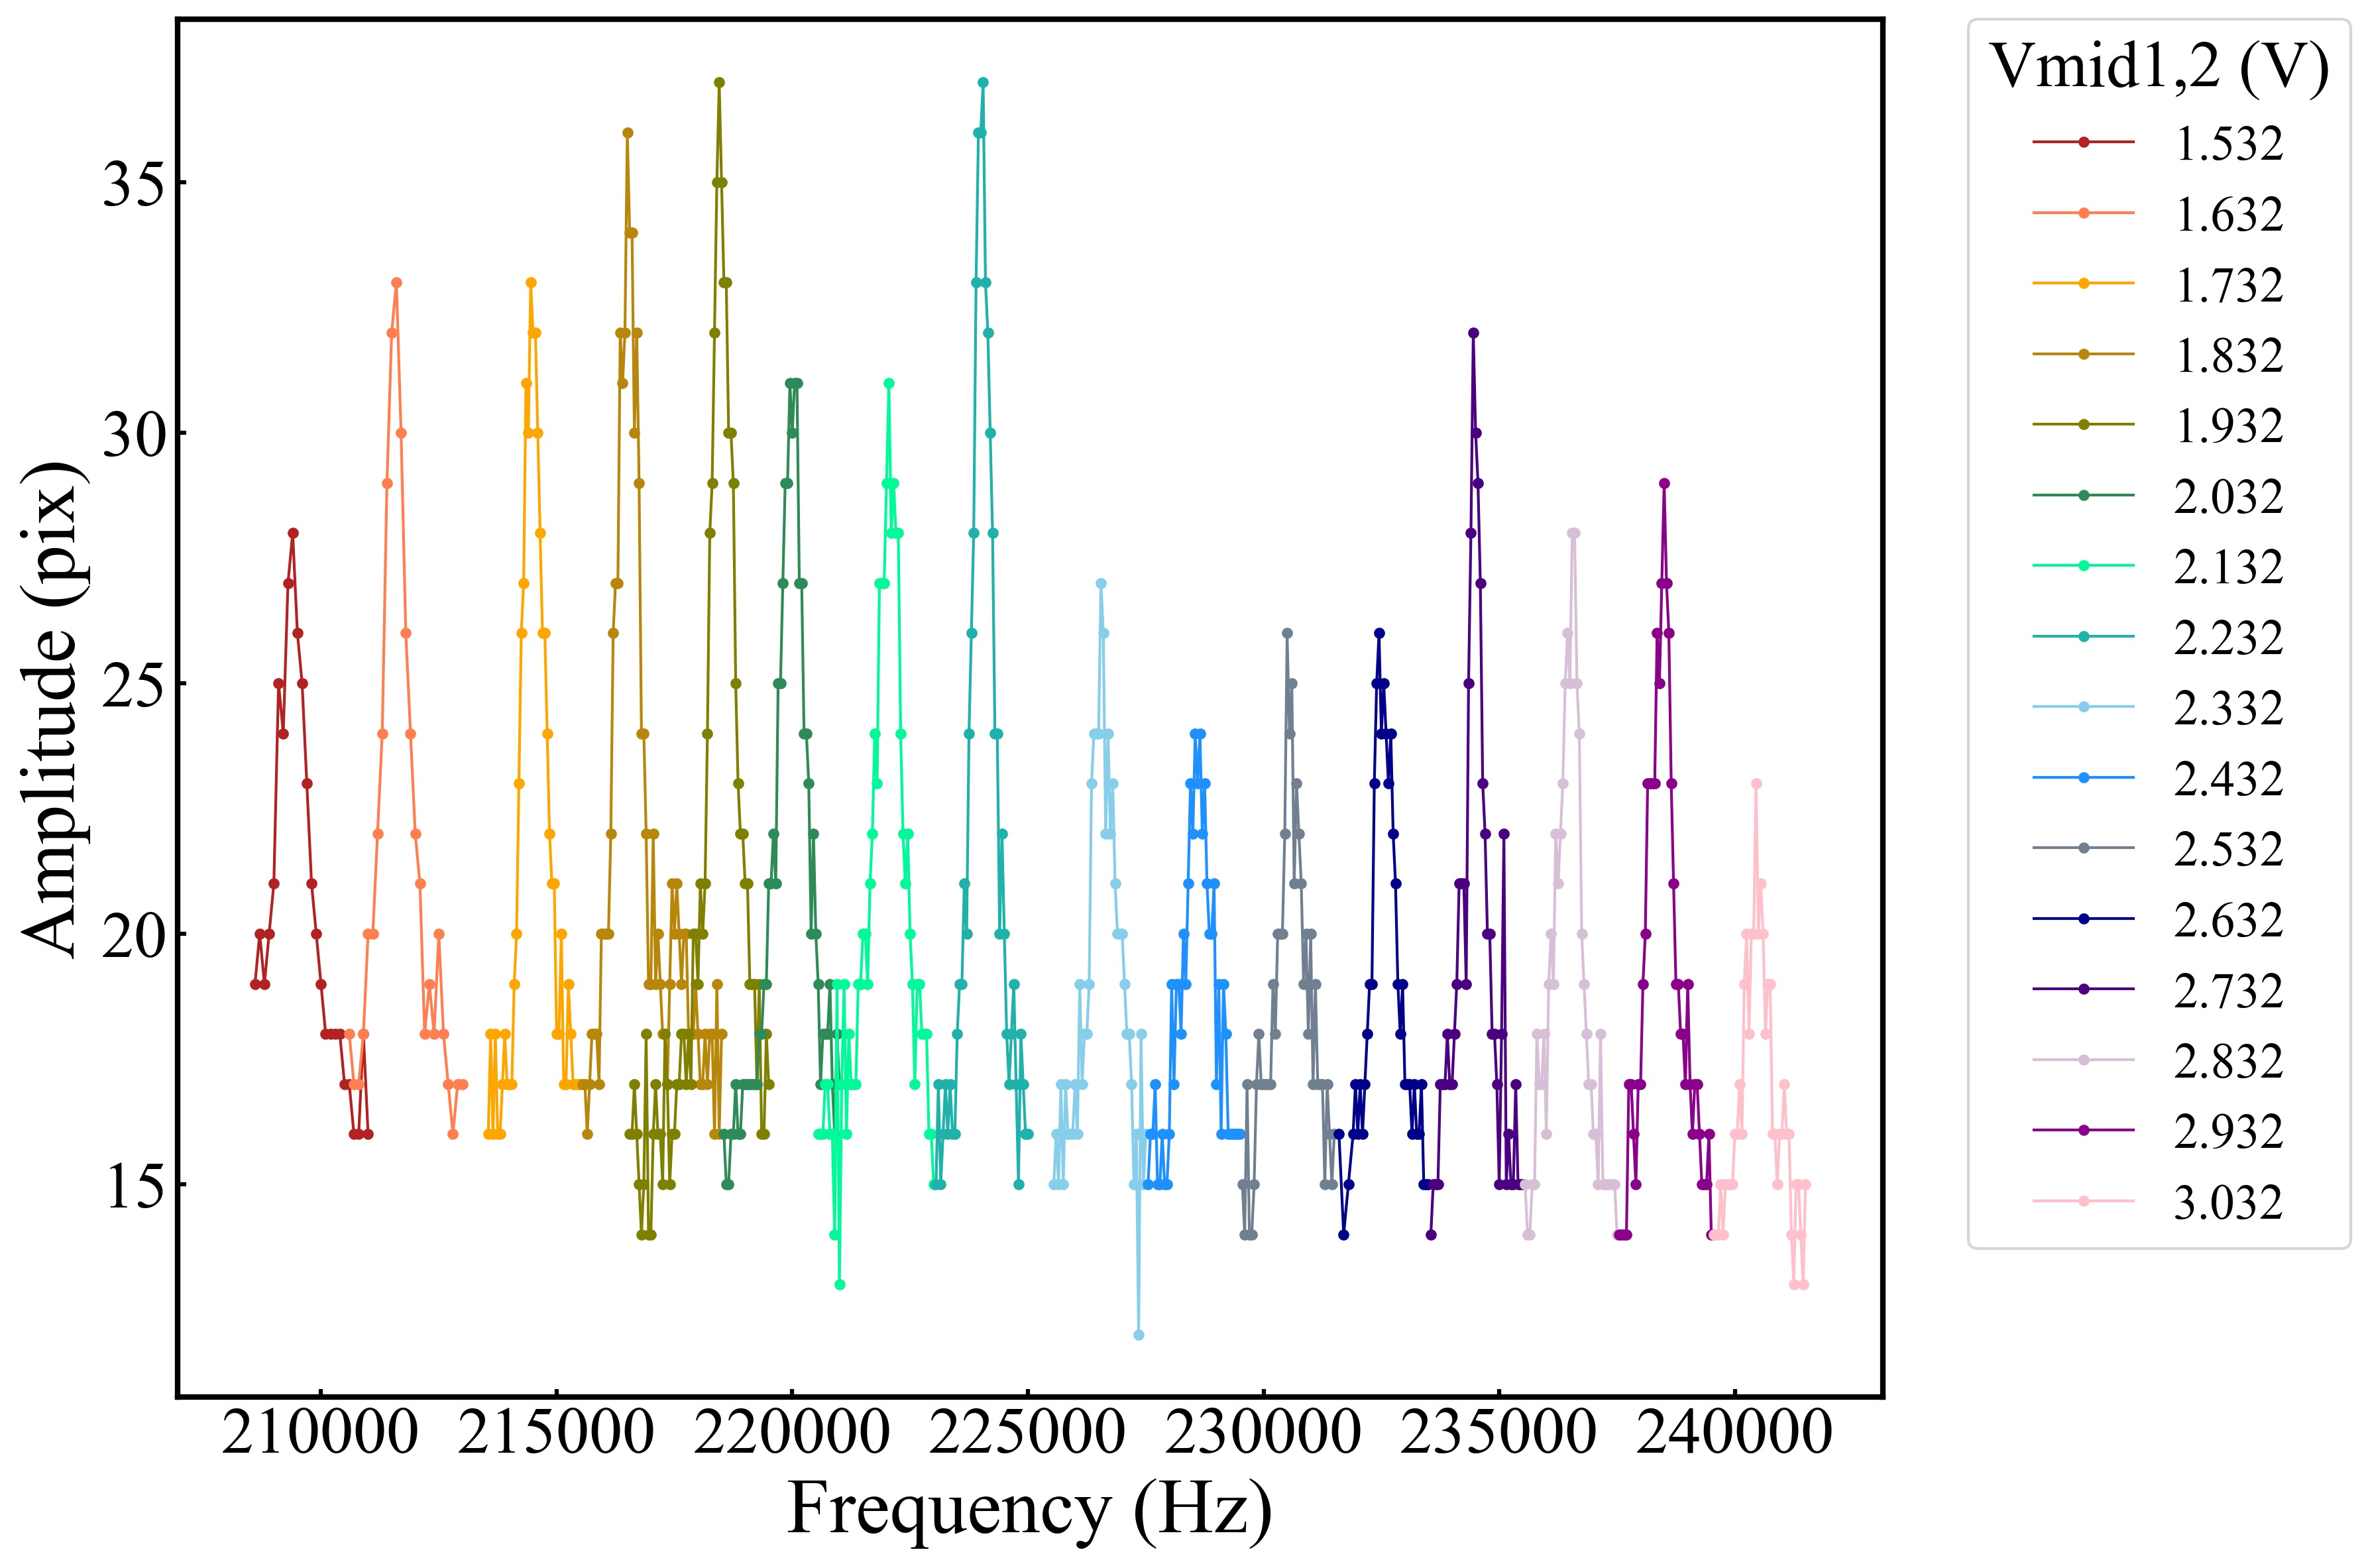
\includegraphics[width = 0.6\linewidth]{./results/figure/mid-SecFreq.jpg}
		\caption{$V_{\rm middle1}$と$V_{\rm middle2}$を変化させたときのイオンの振幅の周波数特性}
		\label{fig:mid_MeasSec}
	\end{center}
\end{figure}

\Fig{mid_MeasSec}からローレンツ分布関数によるフィッティングによって得られる永年周波数とシミュレーションから得られる永年周波数との比較を\Fig{mid12_MeasSec_SimSec}に示す.

\begin{figure}[h]
	\begin{center}
		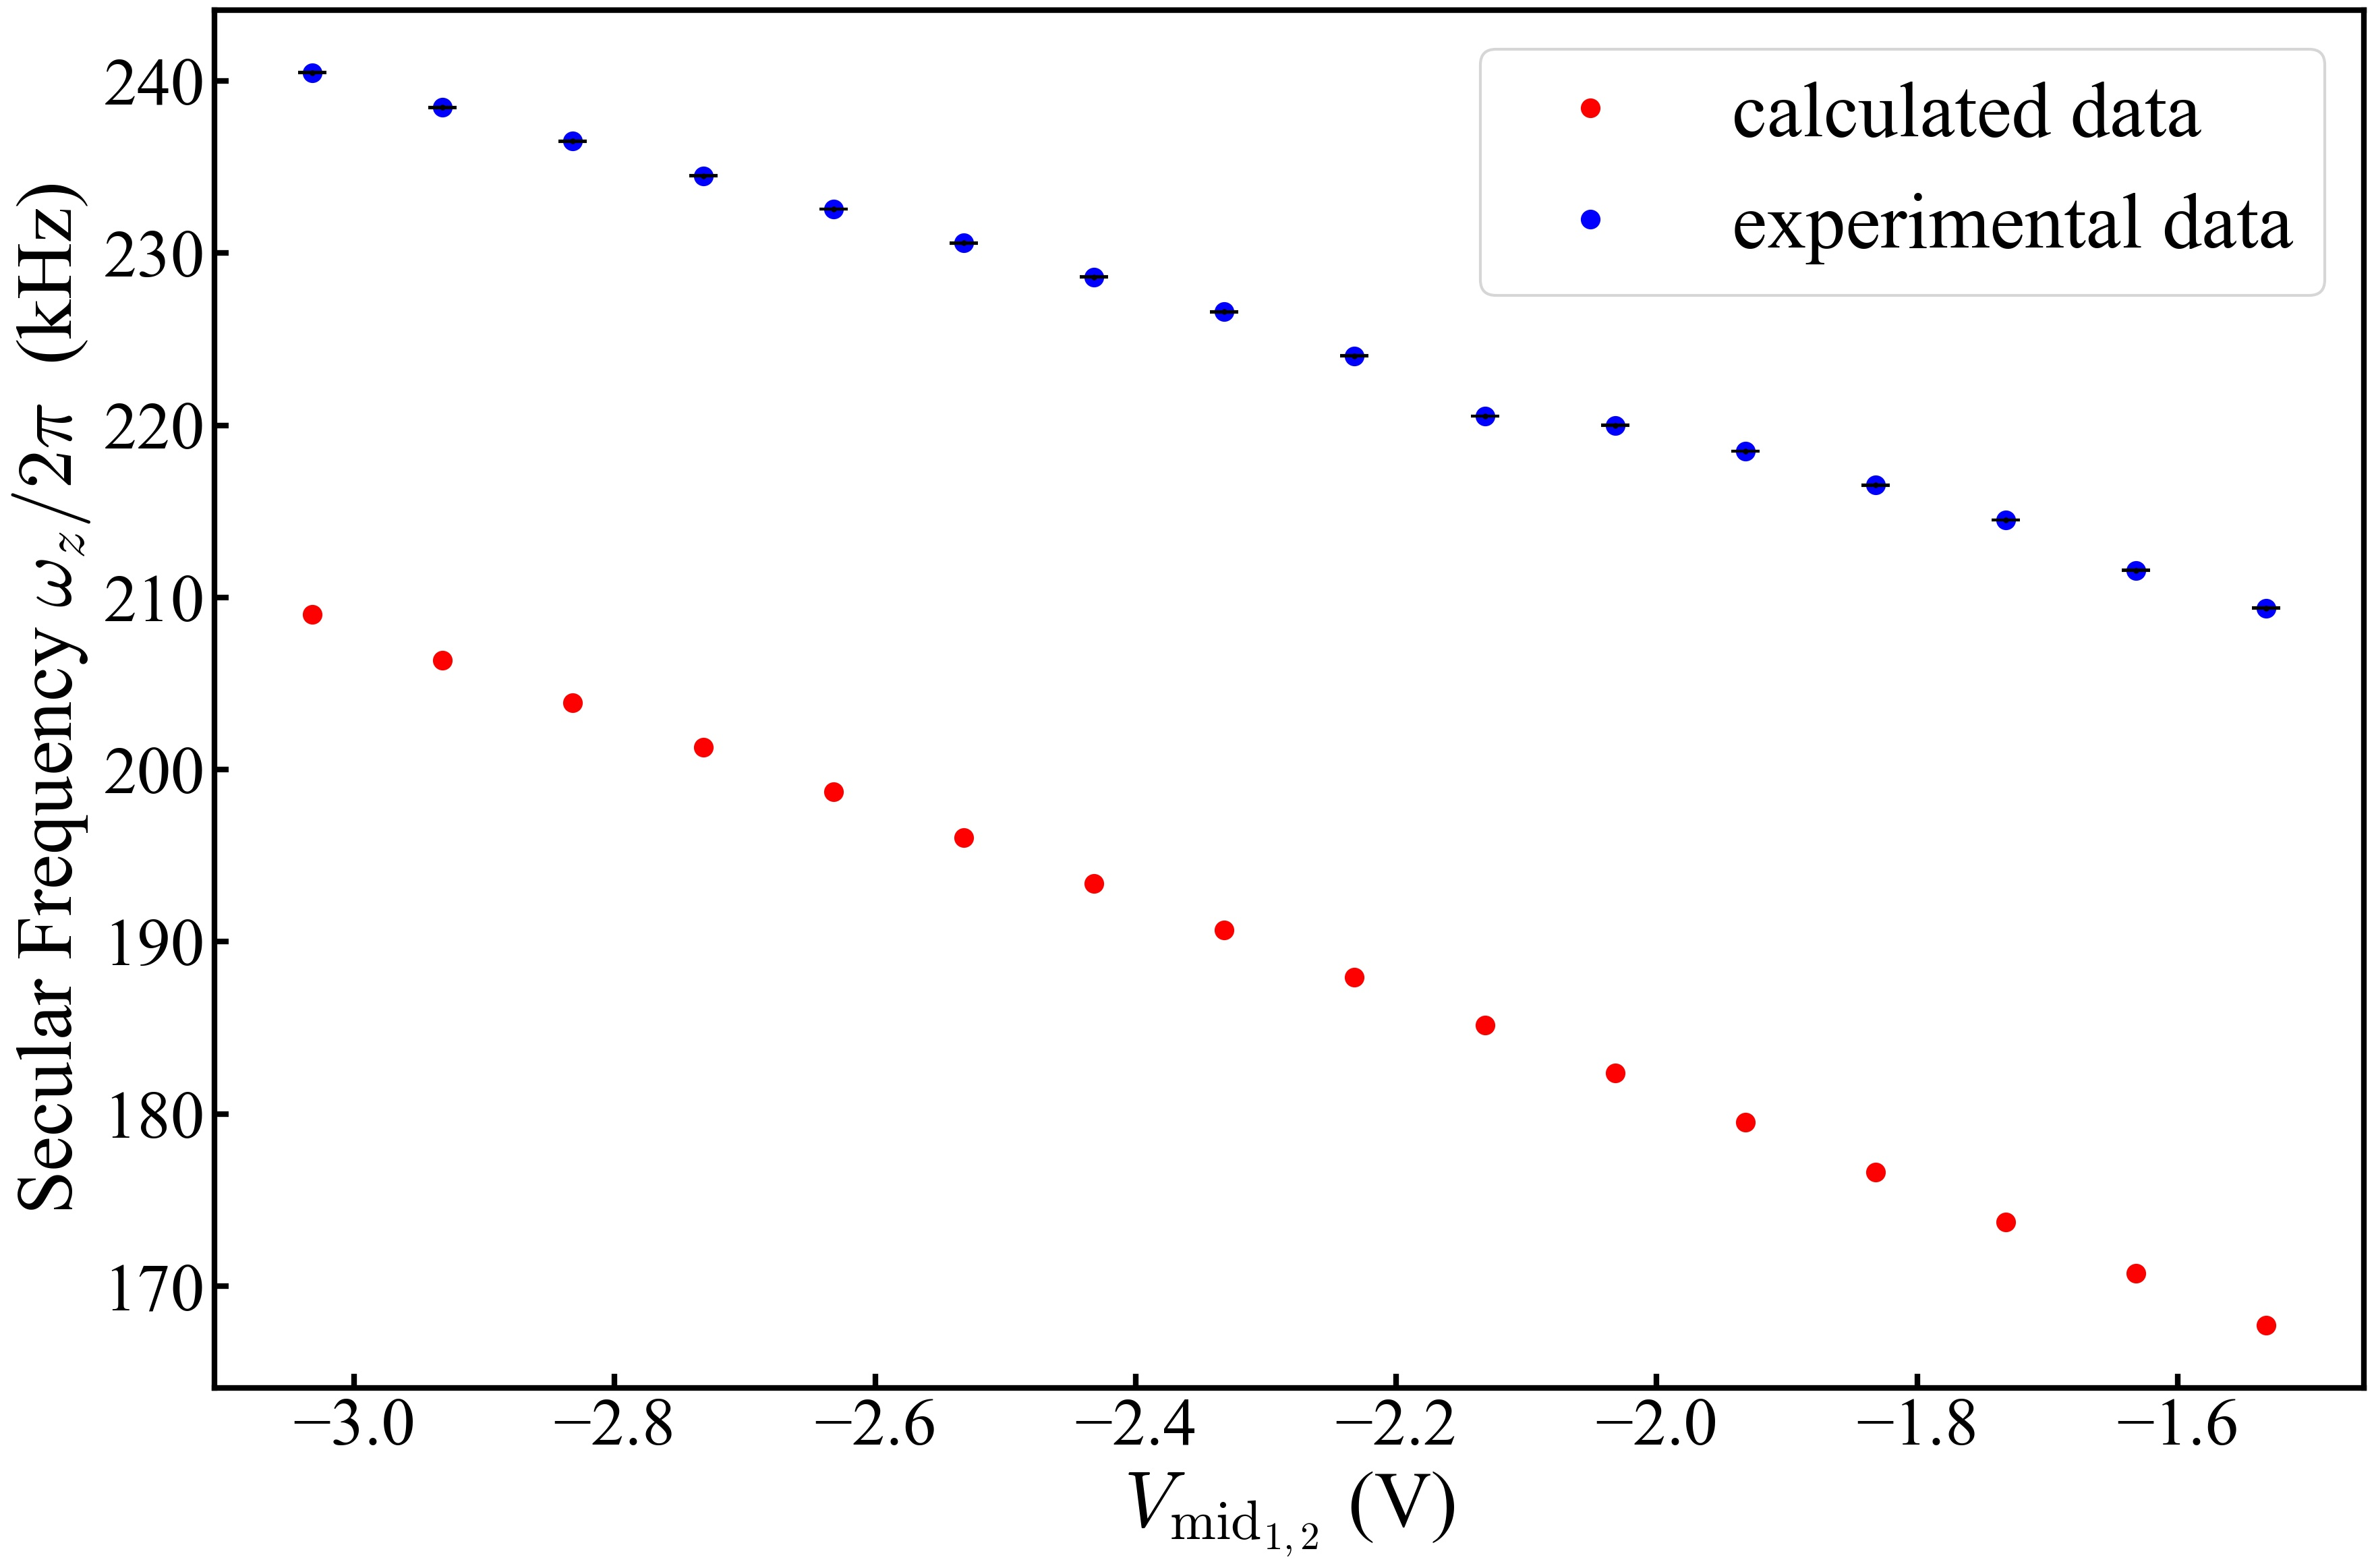
\includegraphics[width = 0.6\linewidth]{./results/figure/Vmid-SecFreqZ.jpg}
		\caption{$V_{\rm middle1}$と$V_{\rm middle2}$を変化させたときの永年周波数の測定結果とシミュレーション結果との比較}
		\label{fig:mid12_MeasSec_SimSec}
	\end{center}
\end{figure}

\Fig{mid12_MeasSec_SimSec}から,実験値とシミュレーション値に$33.2 \ {\rm kHz} \ \sim \ 41.7 \ {\rm kHz}$の差が存在することが分かった.

\clearpage

\section{二列配列イオン}
\subsection{イオン列間距離dと比率Rとの関係}
\subsection{永年周波数の測定結果}

\begin{figure}[h]
	\begin{minipage}{0.5\linewidth}
		\begin{center}
			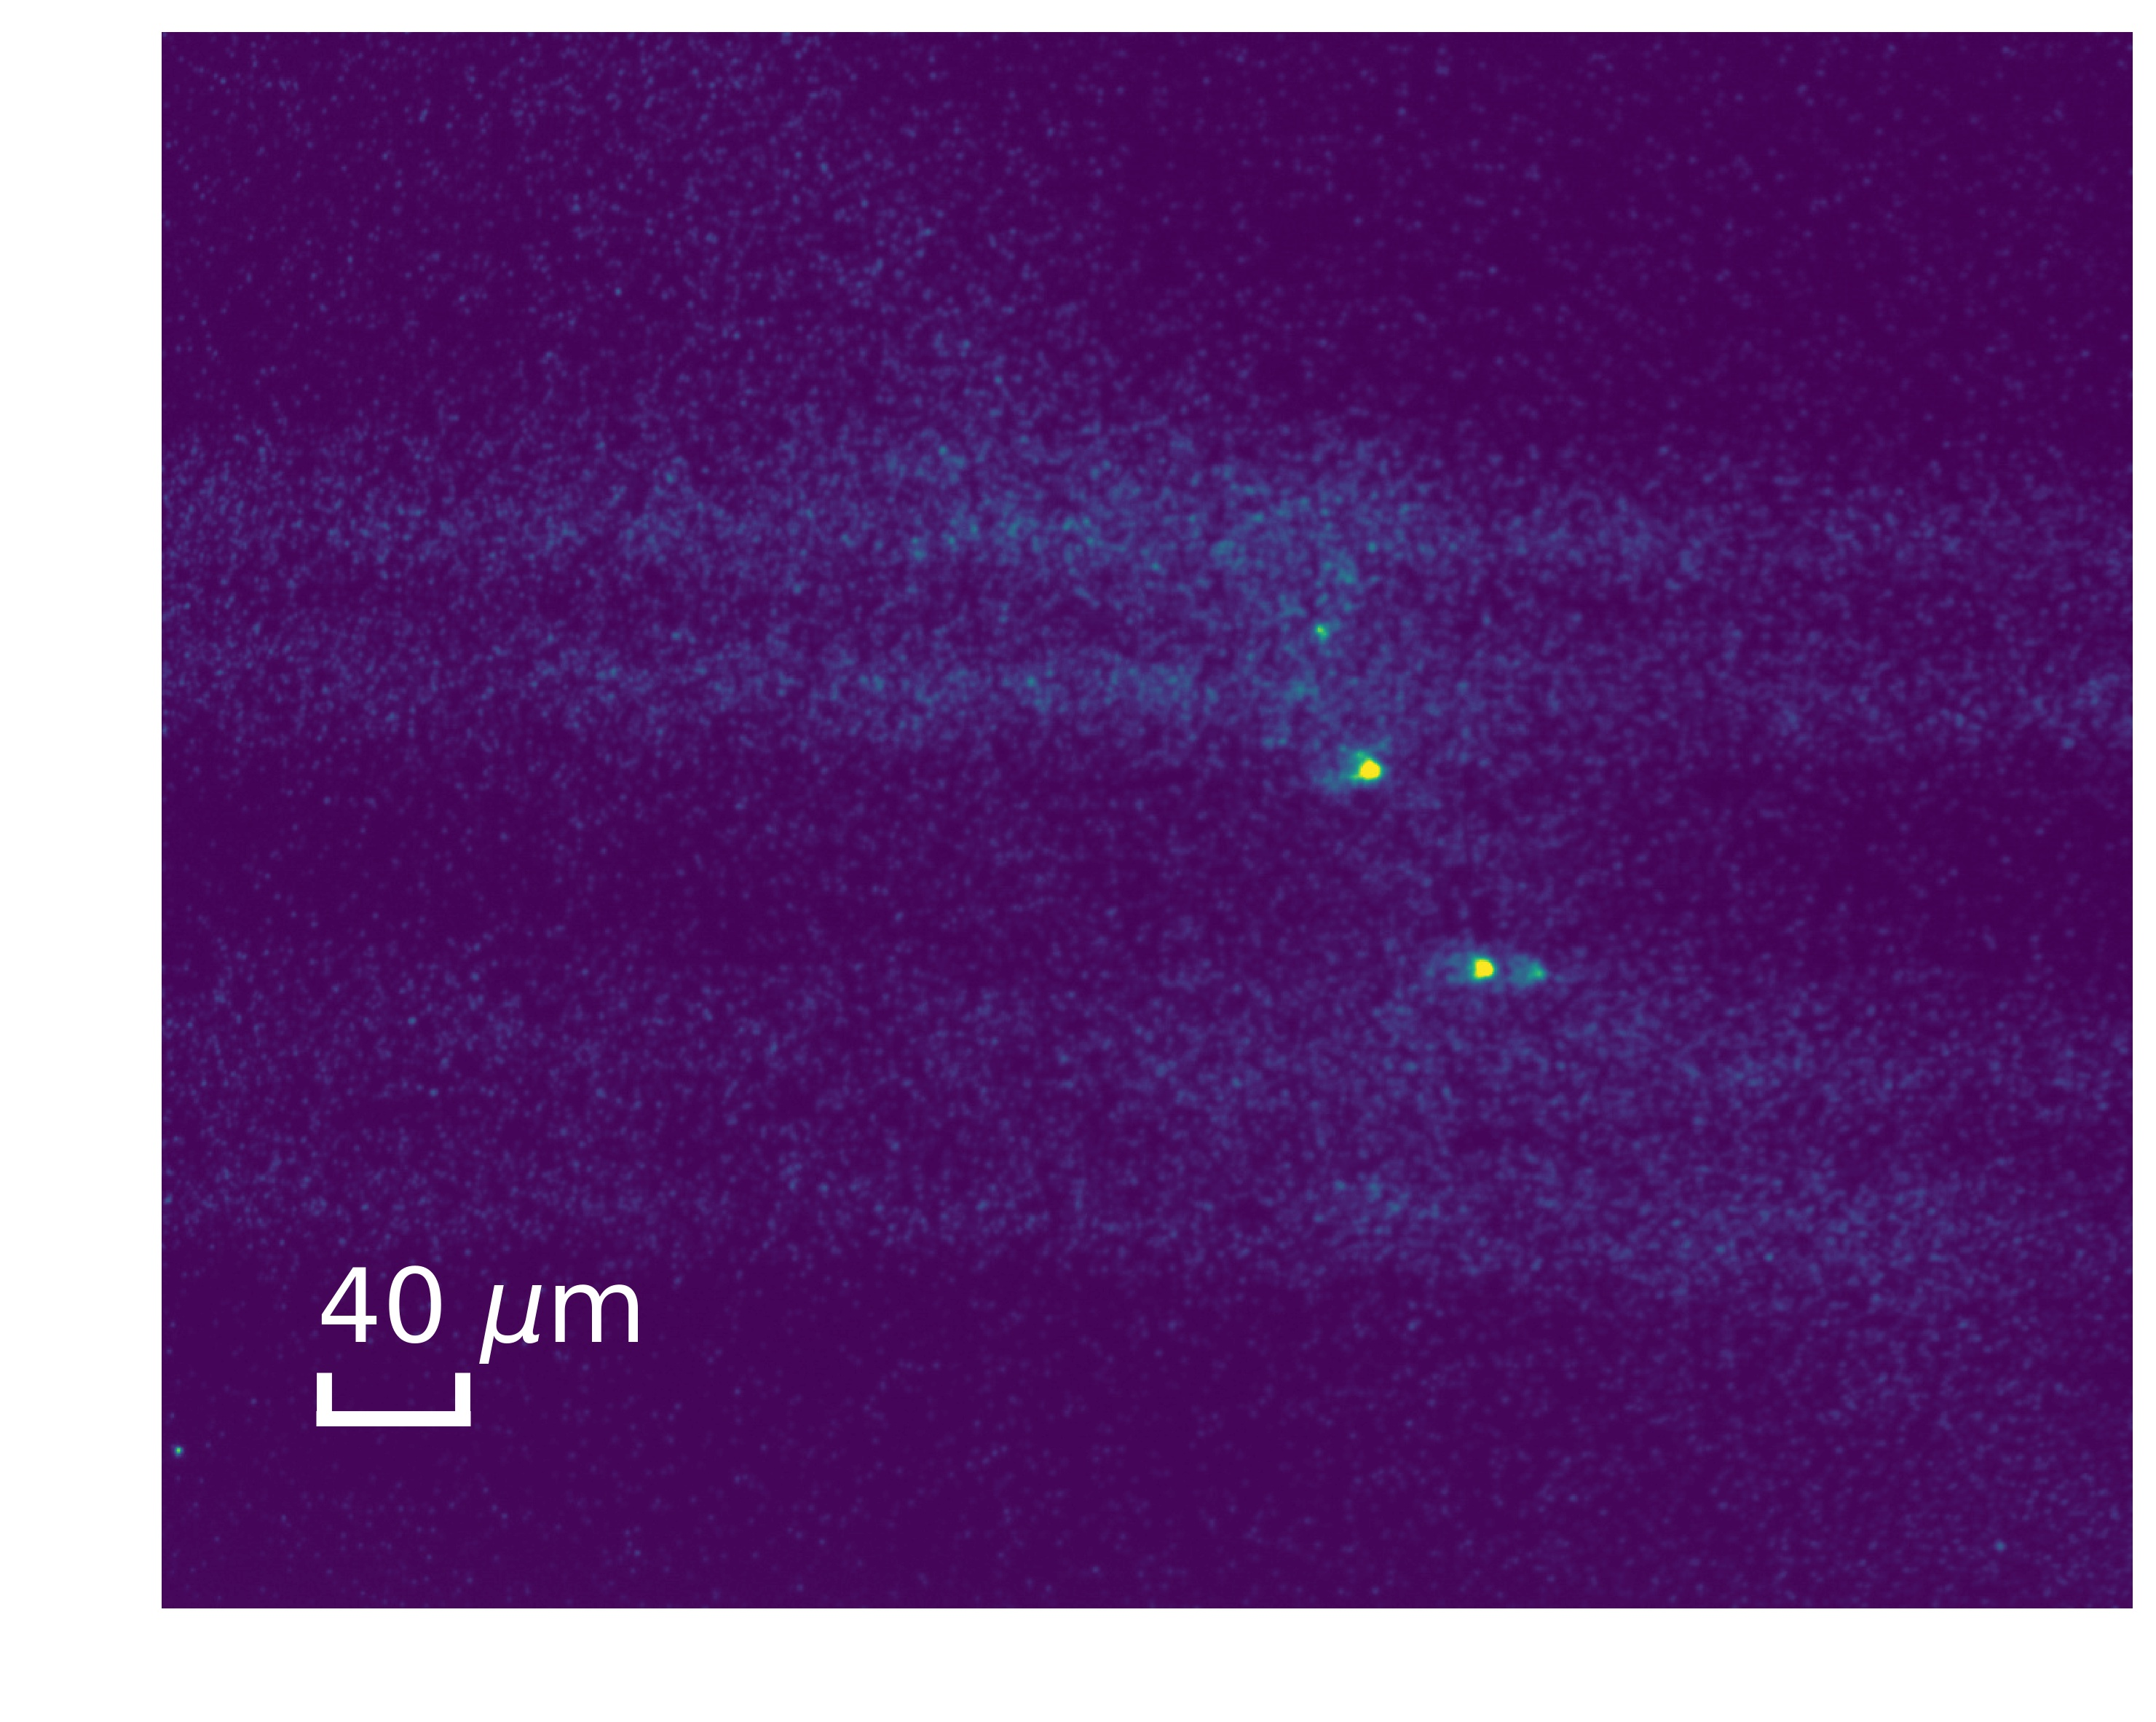
\includegraphics[width = 0.98\columnwidth]{./results/figure/2D_off_resonance.jpg}
			\caption{二列配列イオンでの非共鳴時の捕獲画像}
			\label{fig:2D_off_resonance}
		\end{center}
	\end{minipage}
	\begin{minipage}{0.5\linewidth}
		\begin{center}
			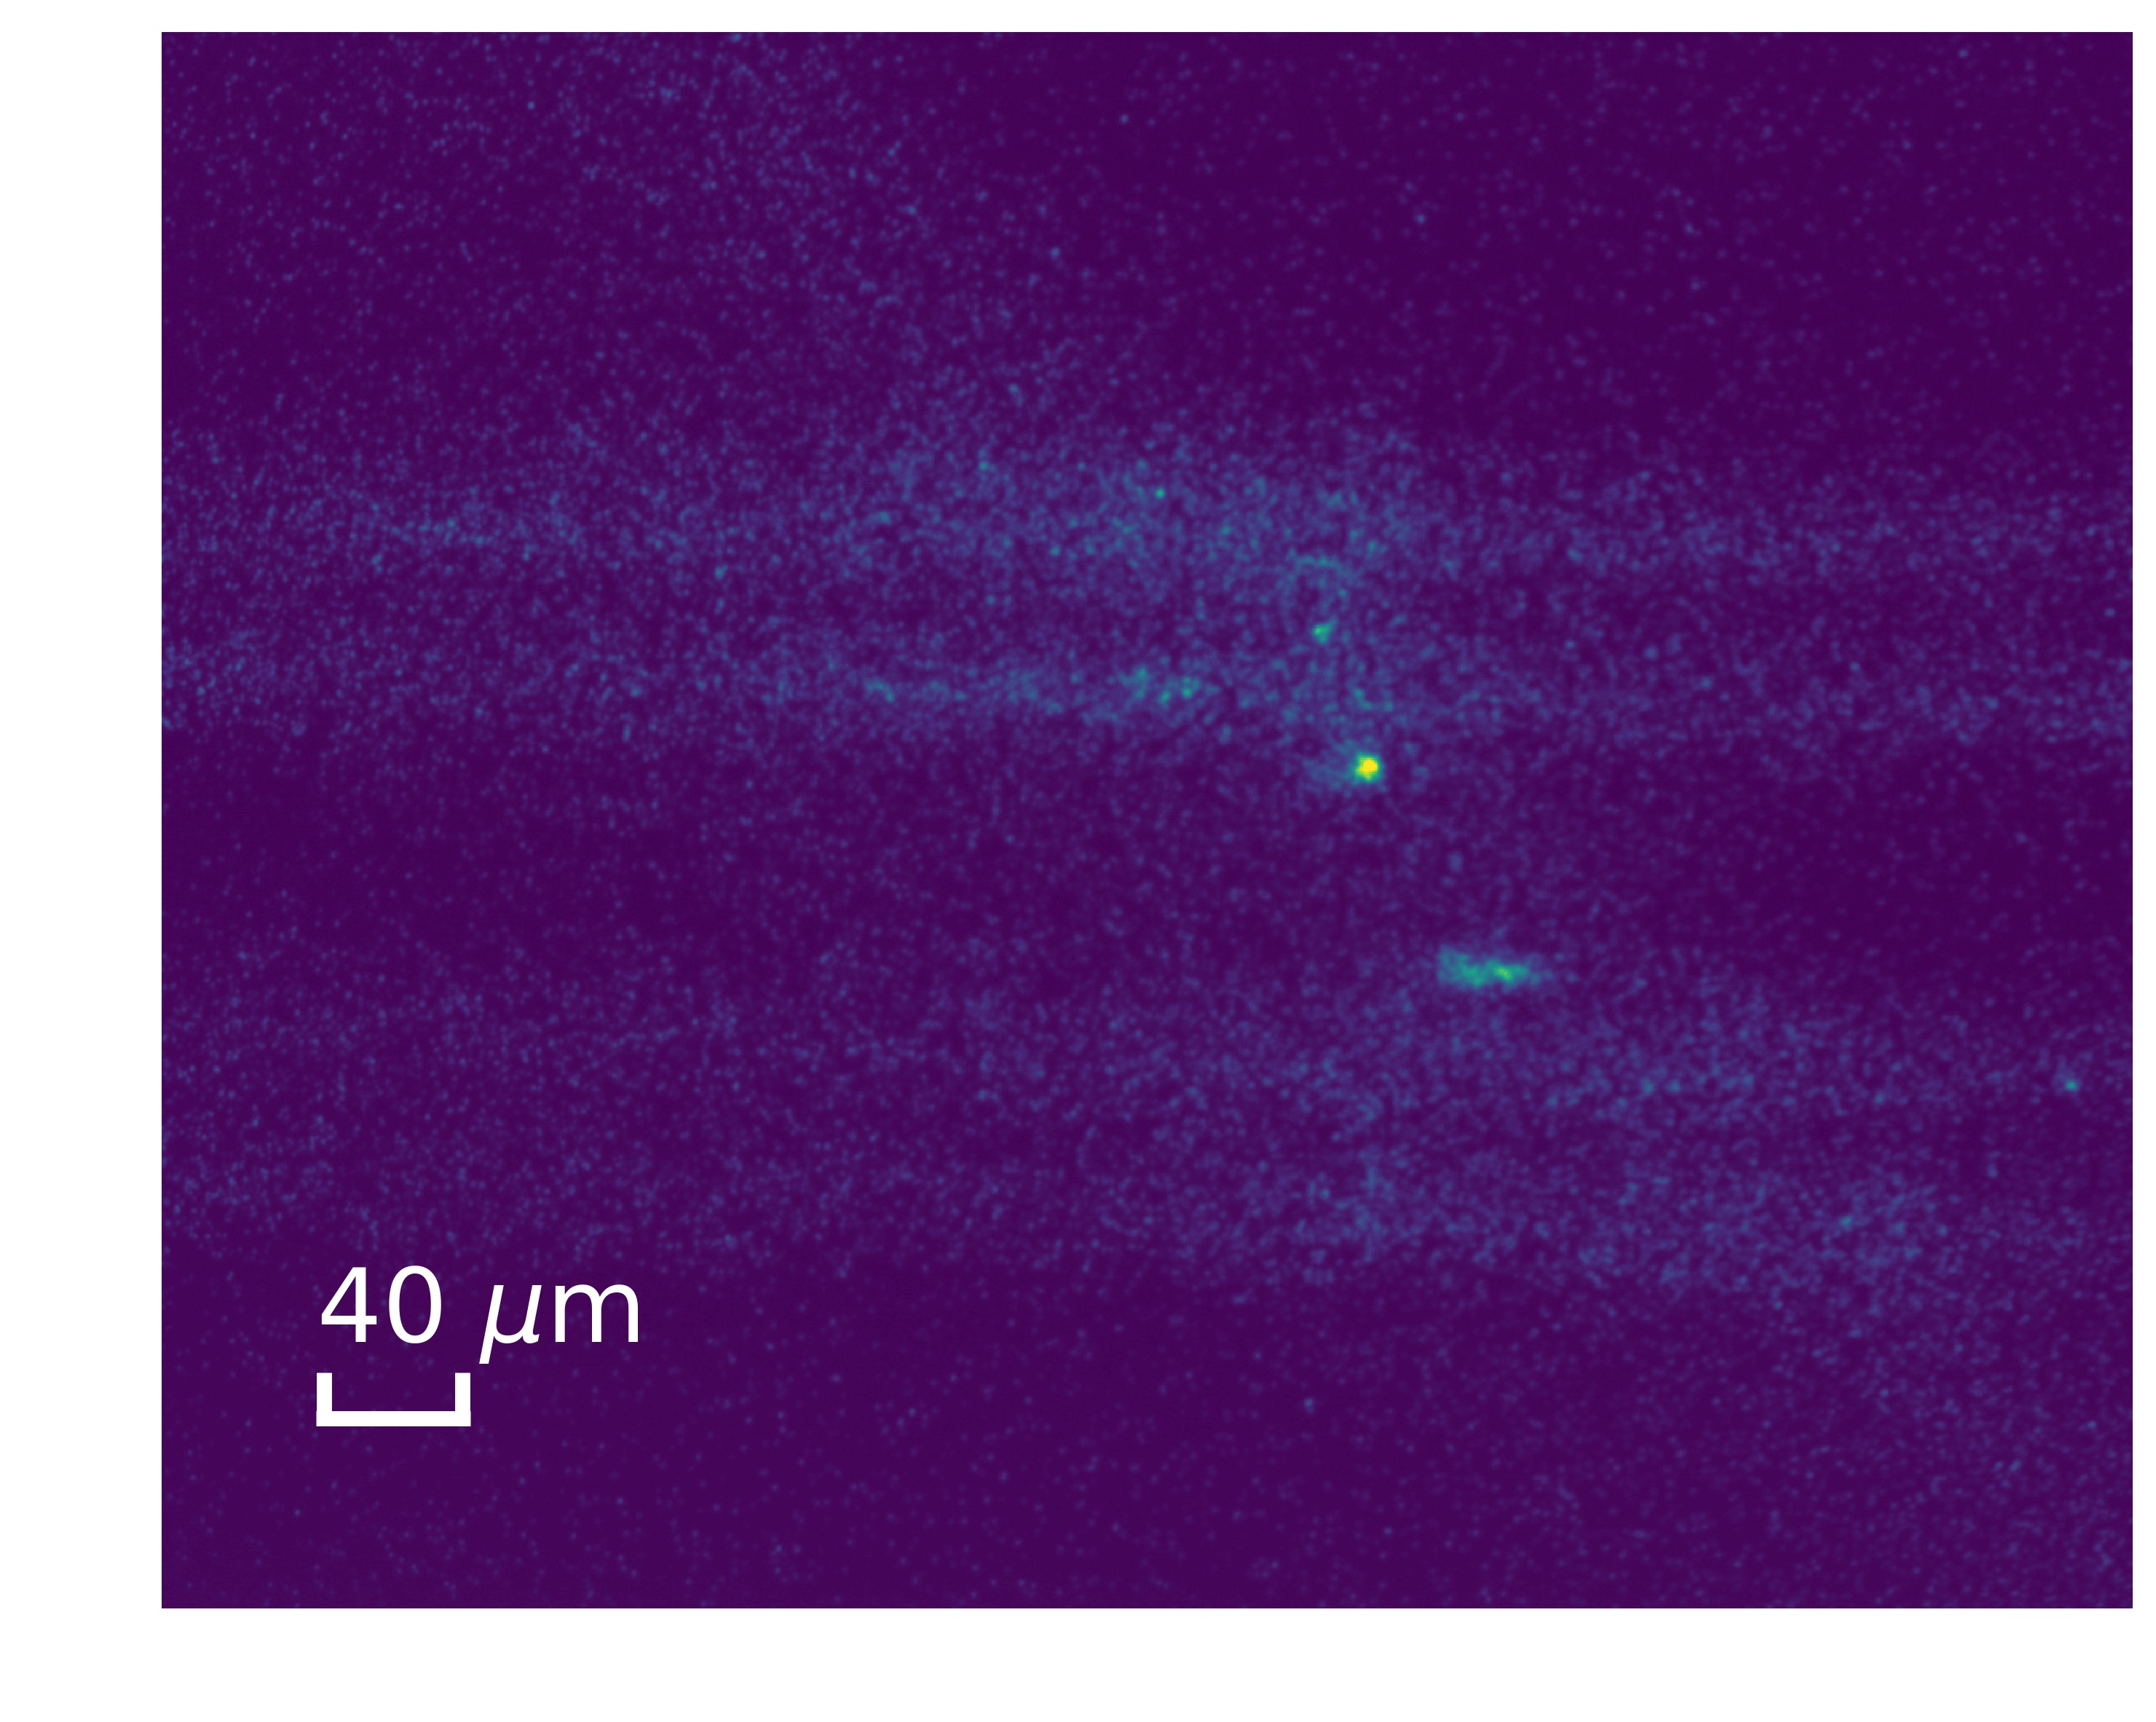
\includegraphics[width = 0.98\columnwidth]{./results/figure/2D_resonance.jpg}
			\caption{二列配列イオンでの共鳴時の捕獲画像}
			\label{fig:2D_resonance}
		\end{center}
	\end{minipage}
\end{figure}